\documentclass{article}
\usepackage{iclr2027_conference,times}
\usepackage[T1]{fontenc}
\usepackage[utf8]{inputenc}
%%%%% NEW MATH DEFINITIONS %%%%%

\usepackage{amsmath,amsfonts,bm}

% Mark sections of captions for referring to divisions of figures
\newcommand{\figleft}{{\em (Left)}}
\newcommand{\figcenter}{{\em (Center)}}
\newcommand{\figright}{{\em (Right)}}
\newcommand{\figtop}{{\em (Top)}}
\newcommand{\figbottom}{{\em (Bottom)}}
\newcommand{\captiona}{{\em (a)}}
\newcommand{\captionb}{{\em (b)}}
\newcommand{\captionc}{{\em (c)}}
\newcommand{\captiond}{{\em (d)}}

% Highlight a newly defined term
\newcommand{\newterm}[1]{{\bf #1}}


% Figure reference, lower-case.
\def\figref#1{figure~\ref{#1}}
% Figure reference, capital. For start of sentence
\def\Figref#1{Figure~\ref{#1}}
\def\twofigref#1#2{figures \ref{#1} and \ref{#2}}
\def\quadfigref#1#2#3#4{figures \ref{#1}, \ref{#2}, \ref{#3} and \ref{#4}}
% Section reference, lower-case.
\def\secref#1{section~\ref{#1}}
% Section reference, capital.
\def\Secref#1{Section~\ref{#1}}
% Reference to two sections.
\def\twosecrefs#1#2{sections \ref{#1} and \ref{#2}}
% Reference to three sections.
\def\secrefs#1#2#3{sections \ref{#1}, \ref{#2} and \ref{#3}}
% Reference to an equation, lower-case.
\def\eqref#1{equation~\ref{#1}}
% Reference to an equation, upper case
\def\Eqref#1{Equation~\ref{#1}}
% A raw reference to an equation---avoid using if possible
\def\plaineqref#1{\ref{#1}}
% Reference to a chapter, lower-case.
\def\chapref#1{chapter~\ref{#1}}
% Reference to an equation, upper case.
\def\Chapref#1{Chapter~\ref{#1}}
% Reference to a range of chapters
\def\rangechapref#1#2{chapters\ref{#1}--\ref{#2}}
% Reference to an algorithm, lower-case.
\def\algref#1{algorithm~\ref{#1}}
% Reference to an algorithm, upper case.
\def\Algref#1{Algorithm~\ref{#1}}
\def\twoalgref#1#2{algorithms \ref{#1} and \ref{#2}}
\def\Twoalgref#1#2{Algorithms \ref{#1} and \ref{#2}}
% Reference to a part, lower case
\def\partref#1{part~\ref{#1}}
% Reference to a part, upper case
\def\Partref#1{Part~\ref{#1}}
\def\twopartref#1#2{parts \ref{#1} and \ref{#2}}

\def\ceil#1{\lceil #1 \rceil}
\def\floor#1{\lfloor #1 \rfloor}
\def\1{\bm{1}}
\newcommand{\train}{\mathcal{D}}
\newcommand{\valid}{\mathcal{D_{\mathrm{valid}}}}
\newcommand{\test}{\mathcal{D_{\mathrm{test}}}}

\def\eps{{\epsilon}}


% Random variables
\def\reta{{\textnormal{$\eta$}}}
\def\ra{{\textnormal{a}}}
\def\rb{{\textnormal{b}}}
\def\rc{{\textnormal{c}}}
\def\rd{{\textnormal{d}}}
\def\re{{\textnormal{e}}}
\def\rf{{\textnormal{f}}}
\def\rg{{\textnormal{g}}}
\def\rh{{\textnormal{h}}}
\def\ri{{\textnormal{i}}}
\def\rj{{\textnormal{j}}}
\def\rk{{\textnormal{k}}}
\def\rl{{\textnormal{l}}}
% rm is already a command, just don't name any random variables m
\def\rn{{\textnormal{n}}}
\def\ro{{\textnormal{o}}}
\def\rp{{\textnormal{p}}}
\def\rq{{\textnormal{q}}}
\def\rr{{\textnormal{r}}}
\def\rs{{\textnormal{s}}}
\def\rt{{\textnormal{t}}}
\def\ru{{\textnormal{u}}}
\def\rv{{\textnormal{v}}}
\def\rw{{\textnormal{w}}}
\def\rx{{\textnormal{x}}}
\def\ry{{\textnormal{y}}}
\def\rz{{\textnormal{z}}}

% Random vectors
\def\rvepsilon{{\mathbf{\epsilon}}}
\def\rvtheta{{\mathbf{\theta}}}
\def\rva{{\mathbf{a}}}
\def\rvb{{\mathbf{b}}}
\def\rvc{{\mathbf{c}}}
\def\rvd{{\mathbf{d}}}
\def\rve{{\mathbf{e}}}
\def\rvf{{\mathbf{f}}}
\def\rvg{{\mathbf{g}}}
\def\rvh{{\mathbf{h}}}
\def\rvu{{\mathbf{i}}}
\def\rvj{{\mathbf{j}}}
\def\rvk{{\mathbf{k}}}
\def\rvl{{\mathbf{l}}}
\def\rvm{{\mathbf{m}}}
\def\rvn{{\mathbf{n}}}
\def\rvo{{\mathbf{o}}}
\def\rvp{{\mathbf{p}}}
\def\rvq{{\mathbf{q}}}
\def\rvr{{\mathbf{r}}}
\def\rvs{{\mathbf{s}}}
\def\rvt{{\mathbf{t}}}
\def\rvu{{\mathbf{u}}}
\def\rvv{{\mathbf{v}}}
\def\rvw{{\mathbf{w}}}
\def\rvx{{\mathbf{x}}}
\def\rvy{{\mathbf{y}}}
\def\rvz{{\mathbf{z}}}

% Elements of random vectors
\def\erva{{\textnormal{a}}}
\def\ervb{{\textnormal{b}}}
\def\ervc{{\textnormal{c}}}
\def\ervd{{\textnormal{d}}}
\def\erve{{\textnormal{e}}}
\def\ervf{{\textnormal{f}}}
\def\ervg{{\textnormal{g}}}
\def\ervh{{\textnormal{h}}}
\def\ervi{{\textnormal{i}}}
\def\ervj{{\textnormal{j}}}
\def\ervk{{\textnormal{k}}}
\def\ervl{{\textnormal{l}}}
\def\ervm{{\textnormal{m}}}
\def\ervn{{\textnormal{n}}}
\def\ervo{{\textnormal{o}}}
\def\ervp{{\textnormal{p}}}
\def\ervq{{\textnormal{q}}}
\def\ervr{{\textnormal{r}}}
\def\ervs{{\textnormal{s}}}
\def\ervt{{\textnormal{t}}}
\def\ervu{{\textnormal{u}}}
\def\ervv{{\textnormal{v}}}
\def\ervw{{\textnormal{w}}}
\def\ervx{{\textnormal{x}}}
\def\ervy{{\textnormal{y}}}
\def\ervz{{\textnormal{z}}}

% Random matrices
\def\rmA{{\mathbf{A}}}
\def\rmB{{\mathbf{B}}}
\def\rmC{{\mathbf{C}}}
\def\rmD{{\mathbf{D}}}
\def\rmE{{\mathbf{E}}}
\def\rmF{{\mathbf{F}}}
\def\rmG{{\mathbf{G}}}
\def\rmH{{\mathbf{H}}}
\def\rmI{{\mathbf{I}}}
\def\rmJ{{\mathbf{J}}}
\def\rmK{{\mathbf{K}}}
\def\rmL{{\mathbf{L}}}
\def\rmM{{\mathbf{M}}}
\def\rmN{{\mathbf{N}}}
\def\rmO{{\mathbf{O}}}
\def\rmP{{\mathbf{P}}}
\def\rmQ{{\mathbf{Q}}}
\def\rmR{{\mathbf{R}}}
\def\rmS{{\mathbf{S}}}
\def\rmT{{\mathbf{T}}}
\def\rmU{{\mathbf{U}}}
\def\rmV{{\mathbf{V}}}
\def\rmW{{\mathbf{W}}}
\def\rmX{{\mathbf{X}}}
\def\rmY{{\mathbf{Y}}}
\def\rmZ{{\mathbf{Z}}}

% Elements of random matrices
\def\ermA{{\textnormal{A}}}
\def\ermB{{\textnormal{B}}}
\def\ermC{{\textnormal{C}}}
\def\ermD{{\textnormal{D}}}
\def\ermE{{\textnormal{E}}}
\def\ermF{{\textnormal{F}}}
\def\ermG{{\textnormal{G}}}
\def\ermH{{\textnormal{H}}}
\def\ermI{{\textnormal{I}}}
\def\ermJ{{\textnormal{J}}}
\def\ermK{{\textnormal{K}}}
\def\ermL{{\textnormal{L}}}
\def\ermM{{\textnormal{M}}}
\def\ermN{{\textnormal{N}}}
\def\ermO{{\textnormal{O}}}
\def\ermP{{\textnormal{P}}}
\def\ermQ{{\textnormal{Q}}}
\def\ermR{{\textnormal{R}}}
\def\ermS{{\textnormal{S}}}
\def\ermT{{\textnormal{T}}}
\def\ermU{{\textnormal{U}}}
\def\ermV{{\textnormal{V}}}
\def\ermW{{\textnormal{W}}}
\def\ermX{{\textnormal{X}}}
\def\ermY{{\textnormal{Y}}}
\def\ermZ{{\textnormal{Z}}}

% Vectors
\def\vzero{{\bm{0}}}
\def\vone{{\bm{1}}}
\def\vmu{{\bm{\mu}}}
\def\vtheta{{\bm{\theta}}}
\def\va{{\bm{a}}}
\def\vb{{\bm{b}}}
\def\vc{{\bm{c}}}
\def\vd{{\bm{d}}}
\def\ve{{\bm{e}}}
\def\vf{{\bm{f}}}
\def\vg{{\bm{g}}}
\def\vh{{\bm{h}}}
\def\vi{{\bm{i}}}
\def\vj{{\bm{j}}}
\def\vk{{\bm{k}}}
\def\vl{{\bm{l}}}
\def\vm{{\bm{m}}}
\def\vn{{\bm{n}}}
\def\vo{{\bm{o}}}
\def\vp{{\bm{p}}}
\def\vq{{\bm{q}}}
\def\vr{{\bm{r}}}
\def\vs{{\bm{s}}}
\def\vt{{\bm{t}}}
\def\vu{{\bm{u}}}
\def\vv{{\bm{v}}}
\def\vw{{\bm{w}}}
\def\vx{{\bm{x}}}
\def\vy{{\bm{y}}}
\def\vz{{\bm{z}}}

% Elements of vectors
\def\evalpha{{\alpha}}
\def\evbeta{{\beta}}
\def\evepsilon{{\epsilon}}
\def\evlambda{{\lambda}}
\def\evomega{{\omega}}
\def\evmu{{\mu}}
\def\evpsi{{\psi}}
\def\evsigma{{\sigma}}
\def\evtheta{{\theta}}
\def\eva{{a}}
\def\evb{{b}}
\def\evc{{c}}
\def\evd{{d}}
\def\eve{{e}}
\def\evf{{f}}
\def\evg{{g}}
\def\evh{{h}}
\def\evi{{i}}
\def\evj{{j}}
\def\evk{{k}}
\def\evl{{l}}
\def\evm{{m}}
\def\evn{{n}}
\def\evo{{o}}
\def\evp{{p}}
\def\evq{{q}}
\def\evr{{r}}
\def\evs{{s}}
\def\evt{{t}}
\def\evu{{u}}
\def\evv{{v}}
\def\evw{{w}}
\def\evx{{x}}
\def\evy{{y}}
\def\evz{{z}}

% Matrix
\def\mA{{\bm{A}}}
\def\mB{{\bm{B}}}
\def\mC{{\bm{C}}}
\def\mD{{\bm{D}}}
\def\mE{{\bm{E}}}
\def\mF{{\bm{F}}}
\def\mG{{\bm{G}}}
\def\mH{{\bm{H}}}
\def\mI{{\bm{I}}}
\def\mJ{{\bm{J}}}
\def\mK{{\bm{K}}}
\def\mL{{\bm{L}}}
\def\mM{{\bm{M}}}
\def\mN{{\bm{N}}}
\def\mO{{\bm{O}}}
\def\mP{{\bm{P}}}
\def\mQ{{\bm{Q}}}
\def\mR{{\bm{R}}}
\def\mS{{\bm{S}}}
\def\mT{{\bm{T}}}
\def\mU{{\bm{U}}}
\def\mV{{\bm{V}}}
\def\mW{{\bm{W}}}
\def\mX{{\bm{X}}}
\def\mY{{\bm{Y}}}
\def\mZ{{\bm{Z}}}
\def\mBeta{{\bm{\beta}}}
\def\mPhi{{\bm{\Phi}}}
\def\mLambda{{\bm{\Lambda}}}
\def\mSigma{{\bm{\Sigma}}}

% Tensor
\DeclareMathAlphabet{\mathsfit}{\encodingdefault}{\sfdefault}{m}{sl}
\SetMathAlphabet{\mathsfit}{bold}{\encodingdefault}{\sfdefault}{bx}{n}
\newcommand{\tens}[1]{\bm{\mathsfit{#1}}}
\def\tA{{\tens{A}}}
\def\tB{{\tens{B}}}
\def\tC{{\tens{C}}}
\def\tD{{\tens{D}}}
\def\tE{{\tens{E}}}
\def\tF{{\tens{F}}}
\def\tG{{\tens{G}}}
\def\tH{{\tens{H}}}
\def\tI{{\tens{I}}}
\def\tJ{{\tens{J}}}
\def\tK{{\tens{K}}}
\def\tL{{\tens{L}}}
\def\tM{{\tens{M}}}
\def\tN{{\tens{N}}}
\def\tO{{\tens{O}}}
\def\tP{{\tens{P}}}
\def\tQ{{\tens{Q}}}
\def\tR{{\tens{R}}}
\def\tS{{\tens{S}}}
\def\tT{{\tens{T}}}
\def\tU{{\tens{U}}}
\def\tV{{\tens{V}}}
\def\tW{{\tens{W}}}
\def\tX{{\tens{X}}}
\def\tY{{\tens{Y}}}
\def\tZ{{\tens{Z}}}


% Graph
\def\gA{{\mathcal{A}}}
\def\gB{{\mathcal{B}}}
\def\gC{{\mathcal{C}}}
\def\gD{{\mathcal{D}}}
\def\gE{{\mathcal{E}}}
\def\gF{{\mathcal{F}}}
\def\gG{{\mathcal{G}}}
\def\gH{{\mathcal{H}}}
\def\gI{{\mathcal{I}}}
\def\gJ{{\mathcal{J}}}
\def\gK{{\mathcal{K}}}
\def\gL{{\mathcal{L}}}
\def\gM{{\mathcal{M}}}
\def\gN{{\mathcal{N}}}
\def\gO{{\mathcal{O}}}
\def\gP{{\mathcal{P}}}
\def\gQ{{\mathcal{Q}}}
\def\gR{{\mathcal{R}}}
\def\gS{{\mathcal{S}}}
\def\gT{{\mathcal{T}}}
\def\gU{{\mathcal{U}}}
\def\gV{{\mathcal{V}}}
\def\gW{{\mathcal{W}}}
\def\gX{{\mathcal{X}}}
\def\gY{{\mathcal{Y}}}
\def\gZ{{\mathcal{Z}}}

% Sets
\def\sA{{\mathbb{A}}}
\def\sB{{\mathbb{B}}}
\def\sC{{\mathbb{C}}}
\def\sD{{\mathbb{D}}}
% Don't use a set called E, because this would be the same as our symbol
% for expectation.
\def\sF{{\mathbb{F}}}
\def\sG{{\mathbb{G}}}
\def\sH{{\mathbb{H}}}
\def\sI{{\mathbb{I}}}
\def\sJ{{\mathbb{J}}}
\def\sK{{\mathbb{K}}}
\def\sL{{\mathbb{L}}}
\def\sM{{\mathbb{M}}}
\def\sN{{\mathbb{N}}}
\def\sO{{\mathbb{O}}}
\def\sP{{\mathbb{P}}}
\def\sQ{{\mathbb{Q}}}
\def\sR{{\mathbb{R}}}
\def\sS{{\mathbb{S}}}
\def\sT{{\mathbb{T}}}
\def\sU{{\mathbb{U}}}
\def\sV{{\mathbb{V}}}
\def\sW{{\mathbb{W}}}
\def\sX{{\mathbb{X}}}
\def\sY{{\mathbb{Y}}}
\def\sZ{{\mathbb{Z}}}

% Entries of a matrix
\def\emLambda{{\Lambda}}
\def\emA{{A}}
\def\emB{{B}}
\def\emC{{C}}
\def\emD{{D}}
\def\emE{{E}}
\def\emF{{F}}
\def\emG{{G}}
\def\emH{{H}}
\def\emI{{I}}
\def\emJ{{J}}
\def\emK{{K}}
\def\emL{{L}}
\def\emM{{M}}
\def\emN{{N}}
\def\emO{{O}}
\def\emP{{P}}
\def\emQ{{Q}}
\def\emR{{R}}
\def\emS{{S}}
\def\emT{{T}}
\def\emU{{U}}
\def\emV{{V}}
\def\emW{{W}}
\def\emX{{X}}
\def\emY{{Y}}
\def\emZ{{Z}}
\def\emSigma{{\Sigma}}

% entries of a tensor
% Same font as tensor, without \bm wrapper
\newcommand{\etens}[1]{\mathsfit{#1}}
\def\etLambda{{\etens{\Lambda}}}
\def\etA{{\etens{A}}}
\def\etB{{\etens{B}}}
\def\etC{{\etens{C}}}
\def\etD{{\etens{D}}}
\def\etE{{\etens{E}}}
\def\etF{{\etens{F}}}
\def\etG{{\etens{G}}}
\def\etH{{\etens{H}}}
\def\etI{{\etens{I}}}
\def\etJ{{\etens{J}}}
\def\etK{{\etens{K}}}
\def\etL{{\etens{L}}}
\def\etM{{\etens{M}}}
\def\etN{{\etens{N}}}
\def\etO{{\etens{O}}}
\def\etP{{\etens{P}}}
\def\etQ{{\etens{Q}}}
\def\etR{{\etens{R}}}
\def\etS{{\etens{S}}}
\def\etT{{\etens{T}}}
\def\etU{{\etens{U}}}
\def\etV{{\etens{V}}}
\def\etW{{\etens{W}}}
\def\etX{{\etens{X}}}
\def\etY{{\etens{Y}}}
\def\etZ{{\etens{Z}}}

% The true underlying data generating distribution
\newcommand{\pdata}{p_{\rm{data}}}
% The empirical distribution defined by the training set
\newcommand{\ptrain}{\hat{p}_{\rm{data}}}
\newcommand{\Ptrain}{\hat{P}_{\rm{data}}}
% The model distribution
\newcommand{\pmodel}{p_{\rm{model}}}
\newcommand{\Pmodel}{P_{\rm{model}}}
\newcommand{\ptildemodel}{\tilde{p}_{\rm{model}}}
% Stochastic autoencoder distributions
\newcommand{\pencode}{p_{\rm{encoder}}}
\newcommand{\pdecode}{p_{\rm{decoder}}}
\newcommand{\precons}{p_{\rm{reconstruct}}}

\newcommand{\laplace}{\mathrm{Laplace}} % Laplace distribution

\newcommand{\E}{\mathbb{E}}
\newcommand{\Ls}{\mathcal{L}}
\newcommand{\R}{\mathbb{R}}
\newcommand{\emp}{\tilde{p}}
\newcommand{\lr}{\alpha}
\newcommand{\reg}{\lambda}
\newcommand{\rect}{\mathrm{rectifier}}
\newcommand{\softmax}{\mathrm{softmax}}
\newcommand{\sigmoid}{\sigma}
\newcommand{\softplus}{\zeta}
\newcommand{\KL}{D_{\mathrm{KL}}}
\newcommand{\Var}{\mathrm{Var}}
\newcommand{\standarderror}{\mathrm{SE}}
\newcommand{\Cov}{\mathrm{Cov}}
% Wolfram Mathworld says $L^2$ is for function spaces and $\ell^2$ is for vectors
% But then they seem to use $L^2$ for vectors throughout the site, and so does
% wikipedia.
\newcommand{\normlzero}{L^0}
\newcommand{\normlone}{L^1}
\newcommand{\normltwo}{L^2}
\newcommand{\normlp}{L^p}
\newcommand{\normmax}{L^\infty}

\newcommand{\parents}{Pa} % See usage in notation.tex. Chosen to match Daphne's book.

\DeclareMathOperator*{\argmax}{arg\,max}
\DeclareMathOperator*{\argmin}{arg\,min}

\DeclareMathOperator{\sign}{sign}
\DeclareMathOperator{\Tr}{Tr}
\let\ab\allowbreak

\usepackage{hyperref}
\usepackage{url}
\usepackage{graphicx}
\usepackage{amsmath,amssymb,amsthm}
\usepackage{booktabs}
\usepackage{multirow}
\usepackage{makecell}
\usepackage{xcolor}
\usepackage{algorithm}
\usepackage[noend]{algpseudocode}
\usepackage{tikz}
\usetikzlibrary{positioning}

\newtheorem{proposition}{Proposition}
\newcommand{\graft}{\textsc{Graft}}
\newcommand{\greater}{\textsc{GReaTer}}
\newcommand{\todo}[1]{\textcolor{red}{[TODO: #1]}}
\providecommand{\R}{\mathbb{R}}

\title{Score Prompt Edits by How They Reshape Reasoning:\\ Distributional Self-Optimization of Structured Prompts}

\author{Anonymous authors\\Paper under double-blind review}

\begin{document}
\maketitle

\begin{abstract}
\greater{} showed that a small language model can optimize its own prompt with the gradient of the
answer loss computed over its own reasoning, one token at a time. Prompts, however, are written and
revised as structured documents. We lift this signal to structural edits---rewriting, deleting and
inserting typed blocks of any length---with an exact calculus in which candidate blocks share one
sequence behind attention gates and rotary slot offsets, so that every vertex is a real edited
prompt. With the signal computable, preregistered experiments on three models show that it ranks
LLM-proposed block edits in the \emph{wrong} direction (8 of 11 proposal pools; as a one-pass
shortlist worse than random in 8 of 11), while fresh evaluation is positive. We trace the failure
to what the gradient is taken over: an edit's effect on accuracy decomposes exactly into a change
of the reasoning distribution and a change of how answers are read off a fixed reasoning, and the
fixed-reasoning objective sees only the second, which on the models' own samples is a small
fraction of the edits' effects, does not predict them, and on wrongly answered questions rewards
reading against the reasoning. Edits move the reasoning distribution by about ten nats per
reasoning, beyond what reweighting the model's own samples by exact likelihood ratios can cover:
this principled repair fails a preregistered test \todo{final numbers}. What edits do must be
observed on fresh reasoning, and verifying candidates on small minibatches chases noise;
\todo{end-to-end: structural search with full verification vs \greater{}; gradient vs random
shortlist inside official \greater{}}.
\end{abstract}

\section{Introduction}
\label{sec:intro}

Automatic prompt optimization is most attractive where it is hardest: for small, locally deployed
models that cannot rely on a stronger model to critique their prompts \citep{zhang2024revisiting}.
\greater{} \citep{das2025greater} showed that such models can optimize their own prompts if the
signal is a true gradient of the task loss computed \emph{over the model's own reasoning}: the
model reasons under the current prompt, an extractor elicits its answer, and the gradient of the
answer loss with respect to one-hot prompt tokens shortlists token substitutions, which are then
verified by regenerating the reasoning.

Token coordinates are a poor match for how prompts are written and reviewed---as structured
documents with a task, a strategy, a procedure and an output contract, edited by rewriting,
deleting or inserting whole instructions. Lifting \greater{}'s signal to such edits poses a
technical problem, since edits of different lengths have no one-hot relaxation, and a conceptual
one: a structural edit changes the very reasoning the gradient is computed over. We solve the
technical problem exactly and then show that the conceptual one is decisive---and that it has a
principled fix.

\textbf{Contributions.}
\begin{itemize}
\item \emph{An exact calculus for structural edits} (\S\ref{sec:calculus}). All candidate rewrites
of all blocks share one sequence in parallel slots behind attention gates, with continuous slot
offsets realized as rotary rotations; every vertex---replacement, deletion, insertion and their
combinations---is exactly a real edited prompt, and one forward/backward pass estimates the effect
of every edit.
\item \emph{A preregistered diagnosis} (\S\ref{sec:diagnosis}). Across three models and eleven
proposal pools, \greater{}'s fixed-reasoning objective ranks LLM-proposed block edits in the wrong
direction ($8$ of $11$ pools; as a one-pass shortlist worse than random in $8$ of $11$), while
fresh evaluation is positive in $9$--$10$ of $11$. Under a deterministic reader, edits rewrite the
reasoning they are scored on, and verifying candidates on small minibatches picks noise.
\item \emph{A decomposition and a fix} (\S\ref{sec:theory}). An edit's effect on accuracy splits
exactly into a reasoning-distribution term and an answer read-off term; the fixed-reasoning
objective sees only the read-off term, which on the models' own samples is three to twenty times
smaller and, on wrongly answered questions, rewards reading against one's own reasoning. Exact
likelihood ratios of the model's own sampled reasoning recover the missing term without
generating under any candidate: \todo{H-dist / H-inc pooled results}.
\item \emph{End-to-end and at scale} (\S\ref{sec:experiments}). \todo{Stage C v2: dist vs
\greater{}-lifted vs random vs textual gradients at matched verification; official \greater{} with
gradient vs random shortlist; breadth over 21 BBH tasks, GSM8K and FOLIO.}
\end{itemize}

\begin{figure*}[t]
\centering
\resizebox{\textwidth}{!}{% Method overview: token-level relaxation (GReaTer) vs superposed typed blocks (GRAFT).
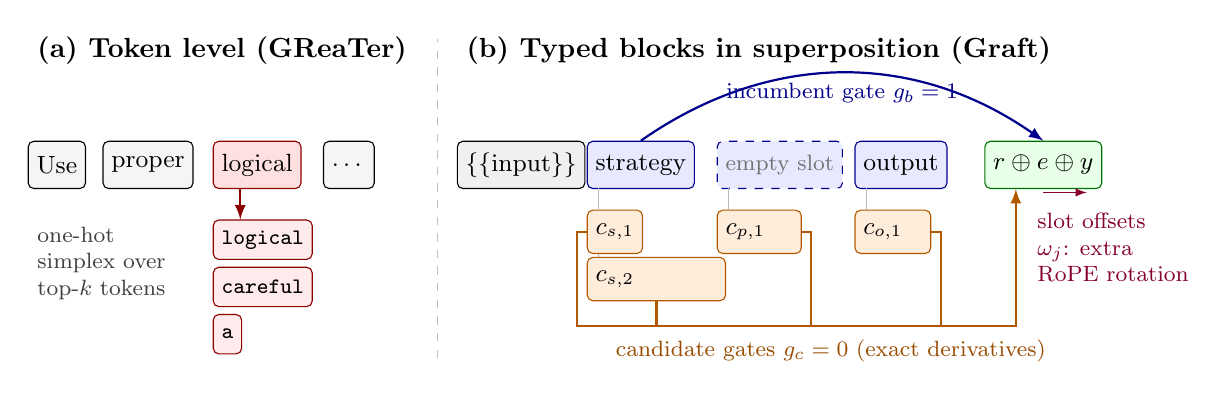
\begin{tikzpicture}[
  x=1cm, y=1cm, font=\small,
  box/.style={draw, rounded corners=2pt, minimum height=6mm, inner sep=3pt, anchor=west},
  tok/.style={box, fill=gray!8},
  alt/.style={box, fill=red!8, draw=red!55!black, minimum height=5mm, font=\footnotesize\ttfamily},
  frz/.style={box, fill=gray!12},
  inc/.style={box, fill=blue!9, draw=blue!55!black},
  cand/.style={box, fill=orange!14, draw=orange!70!black, minimum height=5.5mm},
  tail/.style={box, fill=green!9, draw=green!45!black},
  note/.style={font=\footnotesize, text=black!75, anchor=west, align=left},
  arr/.style={->, >=latex, thick},
]
% ---------------- (a) GReaTer ----------------
\node[anchor=west, font=\bfseries] at (0, 5.05) {(a) Token level (\greater{})};
\node[tok] (u) at (0, 3.6) {Use};
\node[tok] (pr) at (0.95, 3.6) {proper};
\node[tok, fill=red!12, draw=red!55!black] (lo) at (2.35, 3.6) {logical};
\node[tok] (re) at (3.75, 3.6) {\dots};
\node[alt] (a1) at (2.35, 2.65) {logical};
\node[alt] (a2) at (2.35, 2.05) {careful};
\node[alt] (a3) at (2.35, 1.45) {a};
\draw[arr, red!55!black] ([xshift=3.5mm]lo.south west) -- ([xshift=3.5mm]a1.north west);
\node[note] at (0, 2.35) {one-hot\\simplex over\\top-$k$ tokens};

\draw[gray!50, dashed] (5.2, 1.15) -- (5.2, 5.2);

% ---------------- (b) GRAFT ----------------
\node[anchor=west, font=\bfseries] at (5.45, 5.05) {(b) Typed blocks in superposition (\graft{})};
\node[frz] (x) at (5.45, 3.6) {\{\{input\}\}};
\node[inc] (s) at (7.1, 3.6) {strategy};
\node[inc, dashed, text=black!55] (p) at (8.75, 3.6) {\footnotesize empty slot};
\node[inc] (o) at (10.5, 3.6) {output};
\node[tail] (t) at (12.15, 3.6) {$r \oplus e \oplus y$};
% candidate lanes: each starts at its incumbent's first position
\node[cand] (c1) at (7.1, 2.75) {$c_{s,1}$};
\node[cand] (c2) at (7.1, 2.15) {$c_{s,2}$\,\rule{10mm}{0pt}};
\node[cand] (c3) at (8.75, 2.75) {$c_{p,1}$\,\rule{3mm}{0pt}};
\node[cand] (c4) at (10.5, 2.75) {$c_{o,1}$\,\rule{2mm}{0pt}};
\foreach \c in {c1, c3, c4} {\draw[gray!55] ([xshift=1.5mm]\c.north west) -- ++(0, 0.27);}
\draw[gray!55] ([xshift=1.5mm]c2.north west) -- ([xshift=1.5mm]c1.south west);
% incumbent gate
\draw[arr, blue!55!black] (s.north) to[out=35, in=145] node[pos=0.5, below, font=\footnotesize] {incumbent gate $g_b=1$} (t.north);
% candidate gates share a bus into the downstream tokens
\draw[orange!70!black, thick] (c1.west) -- ++(-0.12,0) |- (12.0, 1.55);
\foreach \c in {c3, c4} {\draw[orange!70!black, thick] (\c.east) -- ++(0.12,0) |- (12.0, 1.55);}
\draw[orange!70!black, thick] (c2.south) |- (12.0, 1.55);
\draw[arr, orange!70!black] (12.0, 1.55) -| ([xshift=4mm]t.south west);
\node[font=\footnotesize, text=orange!60!black, anchor=north] at (10.2, 1.5) {candidate gates $g_c=0$ (exact derivatives)};
\node[note, text=purple!70!black] at (12.7, 2.55) {slot offsets\\$\omega_j$: extra\\RoPE rotation};
\draw[->, >=latex, purple!70!black] (12.9, 3.25) -- (13.45, 3.25);
% The vertex and one-pass notes formerly drawn here are stated in the caption and in Section 3.
\end{tikzpicture}
}
\caption{\textbf{From token coordinates to typed blocks.} (a) \greater{} relaxes one prompt token
into the vocabulary simplex; its vertices are real tokens but every edit keeps the prompt's length
and structure. (b) Candidate rewrites of every typed block sit in parallel slots behind attention
gates, with continuous slot offsets realized as rotary rotations; every vertex is exactly a real
edited prompt.}
\label{fig:overview}
\end{figure*}

\section{Setting: self-optimization with gradients over reasoning}
\label{sec:background}

Let $f_\theta$ be a frozen causal language model, $P$ a prompt and $(x,y)$ a question with its gold
answer. Under $P$ the model writes a reasoning $r\sim\pi_P(\cdot\mid x)$ (greedy decoding is the
$\tau\!\to\!0$ limit of temperature-$\tau$ sampling); an extractor $e$ (``Therefore, the final
answer is'') is appended and the answer is read greedily, with correctness $c_P(x,r)\in\{0,1\}$ and
gold-answer probability $q_P(y\mid x,r)=p_\theta(y\mid P(x)\oplus r\oplus e)$. A prompt should
improve its accuracy $J(P)=\mathbb{E}_{x}\,\mathbb{E}_{r\sim\pi_P(\cdot\mid x)}\,c_P(x,r)$.
\greater{} \citep{das2025greater} lets a small model optimize its own prompt. For a training
question it generates the greedy reasoning $\hat r$ under the incumbent prompt and scores a
candidate $P'$ by the answer loss on that \emph{fixed} reasoning,
\begin{equation}
\ell(P';x,y,\hat r)=-\log q_{P'}(y\mid x,\hat r),
\label{eq:greater}
\end{equation}
which we call the \emph{fixed-reasoning objective}. Its gradient with respect to one-hot prompt
tokens ranks the model's own top-$k$ token substitutions; the shortlisted candidates are verified by
regenerating the reasoning on all training questions, and the one with the fewest errors (plus a
small perplexity penalty) is kept. The gradient decides which candidates are tried, fresh reasoning
which is accepted; task and optimizer model coincide. Structural edits (rewrite a block, delete an
instruction, insert a procedure) change the prompt's length, so the one-hot relaxation is undefined.

\section{Exact structural edits in one sequence}
\label{sec:calculus}

A prompt is a sequence of typed blocks $P=(b_1,\dots,b_m)$ (task, strategy, procedure, output,
input, example); editable blocks may be empty insertion slots. The edits of slot $j$ are deletion
and a candidate set $C_j$ proposed by the task model itself from unlabeled training questions
(Appendix~\ref{app:details}). For one question, a single token sequence holds the incumbent prompt
$P(x)$, every candidate of every slot, and a scored tail (the fixed reasoning and answer of
Eq.~\ref{eq:greater}, or a sampled reasoning). Candidate tokens of slot $j$ attend, through the same
gates, to everything before slot $j$ (incumbent blocks and earlier slots' candidates) and to their
own earlier tokens; later tokens attend to the incumbent and to all candidates through gated attention
\begin{equation}
a_{tu}=\frac{G_{tu}\exp(s_{tu}-m_t)}{\sum_{v}G_{tv}\exp(s_{tv}-m_t)},\qquad G_{tu}=g_{\sigma(u)},
\label{eq:gate}
\end{equation}
where $\sigma(u)$ is the segment (incumbent block or candidate) of key $u$; since the gate
multiplies after the max-shift, $g=0$ removes a key exactly. A continuous offset $\omega_j$ per slot
moves every later token by $\Omega_t=\sum_j M_{tj}\omega_j$ positions ($M_{tj}=1$ if token $t$
follows slot $j$, else $0$), as an extra rotary rotation of queries and keys.

\begin{proposition}[Exact vertices]
\label{prop:vertices}
At gates $1$ on incumbents, $0$ on candidates and $\omega=0$, the superposed computation equals
$f_\theta(P(x)\oplus\text{tail})$. Choosing per slot one of \{keep, delete, candidate $c$\}, with
the chosen candidate's gate set to $1$, the replaced incumbent's to $0$ and $\omega_j$ to the
length change ($|c|-|b_j|$, $-|b_j|$, or $|c|$ for an insertion), it equals $f_\theta$ on the
edited prompt, for any number of simultaneous edits of any lengths.
\end{proposition}

The proof is by induction over layers (Appendix~\ref{app:proofs}, where Figure~\ref{fig:overview}
contrasts the construction with \greater{}'s token-level relaxation); fp32 tests confirm it for
Llama, Gemma-2 and Qwen3 architectures, including combined edits (Appendix~\ref{app:tests}).
Because first-order gate derivatives saturate, a one-pass estimator, \emph{renormalized patching},
recomputes downstream attention outputs with slot $j$ swapped and linearizes only later layers
(Eq.~\ref{eq:patch}, Appendix~\ref{app:proofs}; the AtP$^*$ principle of
\citealp{kramar2024atp}): one forward and one backward pass score every single-slot edit.

\section{Do gradients over reasoning predict what structural edits do?}
\label{sec:diagnosis}

\paragraph{Design.} Search succeeds or fails for many reasons, so we test the signal directly.
For a task, a model and an incumbent prompt we draw $24$ training questions and let the model
propose label-free rewrites and insertions for every slot ($20$--$21$ edits per pool). Each
predictor is computed on the $24$ questions; the target is the change in greedy accuracy on $200$
held-out questions. Predictors: \greater{}'s objective (Eq.~\ref{eq:greater}), exactly (one pass
per edited prompt) and by one-pass patching; and, as the evaluation-based reference, fresh greedy
accuracy of every edited prompt on $8$ and on all $24$ questions. Eleven pools: a replication on
Llama-3-8B and Qwen3-8B, three tasks and a non-initial prompt state, with protocol and hypotheses
fixed before its data (v3, eight pools), and a prospective test on an untouched task with three
models (TS3). The validity tasks (logical deduction, tracking shuffled objects) are outside the
benchmark tasks of \S\ref{sec:experiments}. Pools are the units of inference: we report how many
pools agree in sign and an exact sign-flip permutation test over pools; question- and
row-resampling bootstrap intervals are bias-corrected and conditional on the pools. The
split-half reliability $\kappa$ of each held-out target bounds the attainable correlation
(roughly by $\sqrt\kappa$); a best-3 regret---the held-out change of the three truly best edits
minus that of a predictor's top three---measures what a shortlist cares about, against the exact
expectation for a uniformly random shortlist.

\begin{table}[t]
\centering
\caption{\textbf{Spearman correlation between each predictor and the held-out accuracy change of
LLM-proposed block edits} (per pool, pooled mean, and pools agreeing in sign with the sign-flip
test). LD/TS: logical deduction (3/7 objects) and tracking shuffled objects (7); TS3: untouched
task (3 objects). L: Llama-3-8B, Q: Qwen3-8B, G: Gemma-2-9B; $^\ast$ non-initial prompt state;
$\sqrt\kappa$: reliability diagnostic of the held-out target.}
\label{tab:validity}
\resizebox{0.95\textwidth}{!}{\begin{tabular}{lrrrrrrrrrr}
\toprule
Predictor & LD7-L & LD7-L$^\ast$ & LD7-Q & LD7-Q$^\ast$ & LD3-L & LD3-Q & TS7-L & TS7-Q & Pooled & Cost (s) \\
\midrule
Answer loss, exact (\greater{}) & -0.55 & -0.48 & -0.25 & +0.24 & -0.41 & -0.37 & -0.66 & +0.03 & -0.31 [-0.31, -0.10] & 70 \\
Answer loss, patching & -0.54 & -0.59 & -0.12 & +0.39 & -0.05 & -0.30 & -0.42 & +0.02 & -0.20 [-0.28, -0.07] & 94 \\
Fork margin, exact & -0.14 & -0.35 & +0.18 & -0.21 & +0.02 & +0.06 & -0.05 & -0.58 & -0.13 [-0.24, +0.04] & 305 \\
Fork margin, patching & +0.17 & -0.23 & +0.11 & -0.31 & -0.19 & +0.02 & -0.13 & -0.52 & -0.14 [-0.24, +0.07] & 308 \\
Fresh accuracy, 8 rows & +0.48 & -0.07 & +0.18 & +0.34 & +0.27 & +0.38 & +0.48 & -0.30 & +0.22 [+0.01, +0.26] & 537 \\
Fresh accuracy, 24 rows & +0.58 & -0.15 & +0.05 & +0.20 & +0.61 & +0.42 & +0.57 & +0.15 & +0.30 [+0.08, +0.33] & 1190 \\
\midrule
Ceiling $\sqrt{\kappa}$ & 0.56 & 0.76 & 0.61 & 0.11 & 0.88 & 0.84 & 0.95 & 0.80 & & \\
\bottomrule
\end{tabular}
}
\end{table}

\paragraph{The fixed-reasoning objective ranks block edits in the wrong direction.}
\greater{}'s objective correlates negatively with the held-out change in $8$ of $11$ pools
(pooled Spearman $-0.26$; sign-flip $p=0.017$); its one-pass estimate tracks the exact values
(mean Spearman $0.79$ between them) and is negative in $9$ of $11$ pools ($-0.20$; $p=0.037$).
Fresh accuracy on the same questions is positive in $9$ ($8$ questions; $+0.28$, $p=0.010$) and
$10$ ($24$ questions; $+0.33$, $p=0.004$) of the $11$ pools. As a shortlist the patched objective
is worse than a random one in $8$ of $11$ pools (best-3 regret $0.091$ vs.\ $0.067$; $p=0.022$);
the exact objective is not distinguishable from random ($0.075$; worse in $7$ of $11$, $p=0.14$),
and on the untouched task its correlation is null ($-0.13$) rather than negative. The direction
is consistent across models and tasks; its size is not. Splitting training questions by whether
the incumbent answers them correctly, and ranking each question's loss changes across edits
before averaging (which removes scale differences between questions), the negative correlation
on wrongly answered questions persists for Llama-3 ($-0.25$ to $-0.61$ in all five pools) but not
for Qwen3 ($+0.25$, $-0.04$, $+0.07$): the unfaithful-read mechanism of
Proposition~\ref{prop:faithful} explains a model-dependent part of the failure, the absence of the
distribution term explains the rest. Two preregistered repairs---a decision margin at reasoning
forks and the objective restricted to correctly answered questions---failed their criteria
(Appendix~\ref{app:prereg}).

\paragraph{Edits rewrite the reasoning, even token edits.} The fixed reasoning is the weak point.
Under a reader that we verified to be deterministic (three re-reads of the same prompt give
token-identical reasoning on $200$ questions; the answer read differs on $0$--$0.5\%$), a single
\greater{}-style token substitution \todo{deterministic re-roll numbers: reasoning changed on X\%,
first divergence after Y tokens, correctness flipped on Z\%}, while net accuracy moves by about
$\pm2$ points; at this granularity no predictor, gradient or evaluation, is distinguishable from
zero on $200$ questions (Appendix~\ref{app:results}).

\begin{table}[t]
\centering
\caption{\textbf{Where an edit's effect lives} (Eq.~\ref{eq:decomp}, estimated on the incumbent's
$16$ samples per training question). Read-off flips: fraction of (candidate, question, sample)
whose hard read of the same reasoning changes; $|A|$, $|D|$: mean absolute read-off and
reasoning-distribution terms per edit (accuracy points$/100$); sd of the log-likelihood ratios.}
\label{tab:readoff}
\small
\begin{tabular}{lrrrr}
\toprule
Pool & Read-off flips & $|A|$ & $|D|$ & sd$(\log w)$ \\
\midrule
LD7, L$^\ast$ & 3.2\% & 0.012 & 0.034 & 43.5 \\
LD7, L & 1.4\% & 0.005 & 0.039 & 19.6 \\
LD3, L & 0.2\% & 0.002 & 0.041 & 19.0 \\
\bottomrule
\end{tabular}

\end{table}

\paragraph{Verification noise.} Self-optimization loops shortlist candidates and verify them by
fresh accuracy on training questions. Simulating one round on each pool with the recorded
per-question correctness, accepting the best of all candidates by fresh accuracy on $8$ questions
\emph{lowers} held-out accuracy by $2.3$ points on average (on $16$ questions $-0.8$, on $24$
$+1.1$), while the best edit of each pool would add $5.5$: on small minibatches verification picks
noise. \greater{} verifies on all its training questions; the structural search of
\S\ref{sec:experiments} does the same.

\section{What a fixed-reasoning gradient can and cannot see}
\label{sec:theory}

An edit $P\to P'$ changes accuracy (Eq.~\ref{eq:J}) through two channels: the reasoning the model
writes, and how an answer is read off a given reasoning. With the likelihood ratio of a reasoning
under the two prompts, $w(r)=\pi_{P'}(r\mid x)/\pi_P(r\mid x)$, and $\mathbb{E}_{\pi_P}[w\,g]=\mathbb{E}_{\pi_{P'}}[g]$,
\begin{equation}
J(P')-J(P)=\underbrace{\mathbb{E}_{x}\mathbb{E}_{r\sim\pi_P}\big[(w(r)-1)\,c_{P'}(x,r)\big]}_{D\text{: reasoning distribution}}
+\underbrace{\mathbb{E}_{x}\mathbb{E}_{r\sim\pi_P}\big[c_{P'}(x,r)-c_P(x,r)\big]}_{A\text{: answer read-off}} .
\label{eq:decomp}
\end{equation}
This identity is exact (for $\tau>0$, where every reasoning has positive probability under both
prompts). \greater{}'s objective (Eq.~\ref{eq:greater}) is a soft version of the read-off term $A$
evaluated on a single reasoning, the incumbent's greedy trace, and its gradient is the first-order
change of that quantity; it carries no information about $D$. To first order in a small edit,
$D\approx\operatorname{Cov}_{\pi_P}(\log w,\,c)$: an edit helps if it makes the model's own
\emph{correct} reasoning more likely relative to its incorrect reasoning---the score-function
term that a gradient taken over a fixed reasoning drops.

\begin{proposition}[Faithful reading]
\label{prop:faithful}
If, for every candidate $P'$, the answer read under $P'$ equals the answer read under $P$ except
on a set of reasonings of $\pi_P$-probability at most $\varepsilon$, then $|A|\le\varepsilon$ and
$J(P')-J(P)=D\pm\varepsilon$. Moreover, on a question whose reasoning $r$ supports a wrong answer
$a\neq y$, every decrease of \greater{}'s loss on $r$ raises the probability of reading an answer
that the reasoning does not support, and a decrease by $\delta>0$ nats implies
$q_{P'}(a\mid x,r)\le1-e^{\delta}q_P(y\mid x,r)$.
\end{proposition}

The proof is immediate from Eq.~\ref{eq:decomp} and $q_{P'}(a\mid x,r)+q_{P'}(y\mid x,r)\le1$.
The regime is not hypothetical. Measured directly on the incumbents' own samples (no weights
involved), the hard read of a fixed reasoning changes under a candidate in only $0.2$--$3.2\%$ of
(candidate, question, sample) triples; the read-off term is $0.1$--$1.2$ accuracy points per edit,
against held-out effects of $3.4$--$10.9$ points, and it does not predict them (Spearman $-0.31$ to
$+0.28$; Table~\ref{tab:readoff}). Two consequences follow. First, a signal computed on a fixed
reasoning measures a small and, on wrongly answered questions, unfaithful part of an edit's effect
(\S\ref{sec:diagnosis} finds exactly this signature). Second, edits move the reasoning
distribution far: the divergence $\mathrm{KL}(\pi_P\,\|\,\pi_{P'})=-\mathbb{E}_{\pi_P}[\log w]$ has a
median of $4.5$--$14.6$ nats per reasoning across pools, so the reasoning a fixed-trace gradient is
taken over is rarely a likely reasoning under the edited prompt.

\paragraph{The natural repair: reweight the model's own samples.} If the missing term is $D$,
the obvious fix keeps \greater{}'s white-box access and estimates $D$ from samples drawn once
under the incumbent. Sample $r_1,\dots,r_S\sim\pi_P^\tau(\cdot\mid x)$ per training question,
read them under the incumbent, and compute for every candidate the exact log-ratios $\log w_s$ of
the \emph{same} samples (teacher forcing, or one superposed pass, \S\ref{sec:calculus}). The
tempered self-normalized importance estimate
\begin{equation}
\widehat{J}_\beta(P'\mid x)=\frac{\sum_s w_s^{\beta}\,c_P(x,r_s)}{\sum_s w_s^{\beta}},\qquad
\widehat{\Delta}_\beta(P')=\mathbb{E}_x\big[\widehat{J}_\beta(P'\mid x)-\tfrac1S\textstyle\sum_s c_P(x,r_s)\big]
\label{eq:snis}
\end{equation}
estimates $D$ (with candidate reads $c_{P'}$ instead of $c_P$ it estimates the full change).
$\beta=0$ recovers the fixed-reasoning family (no reweighting); $\beta=1$ is consistent as
$S\to\infty$; intermediate $\beta$ trades bias for variance, and for small $\beta$,
$\widehat\Delta_\beta\approx\beta\,\widehat{\operatorname{Cov}}(\log w,c)$. Because importance
weights over hundreds of tokens are heavy-tailed, we choose $\beta$ \emph{without labels} as the
largest value in $\{1,\tfrac12,\tfrac14\}$ whose median effective sample size
$(\sum_s w_s^\beta)^2/\sum_s w_s^{2\beta}$ is at least $S/4$. No reasoning is generated and no
answer is read under any candidate. The catch is coverage: importance sampling needs a sample of
size about $\exp(\mathrm{KL})$ between target and proposal \citep{chatterjee2018sample}, and the
divergences measured above are around ten nats per reasoning. Self-normalization hides this---the
weights are renormalized among samples that are all unlikely under the candidate---so the estimate
can look well-conditioned while measuring nothing. We nevertheless test it, preregistered, because
it is the principled ``gradient over the distribution of reasoning'' that \greater{}'s objective
lacks (\S\ref{sec:exp-validity}).

\paragraph{Why verification is noisy.} Greedy correctness is a $\{0,1\}$ quantization of a
per-question success probability. Comparing two prompts on $n$ questions by greedy accuracy has
variance $\approx f/n$, where $f$ is the fraction of questions whose correctness flips between
them; single edits flip $16$--$22\%$ of questions while moving accuracy by about two points
(\S\ref{sec:diagnosis}), so on an $8$-question minibatch the comparison has a standard deviation of
about $15$ points. Selecting the best of many candidates on such a comparison is a winner's curse.

\section{Distributional self-optimization of structured prompts}
\label{sec:method}

\begin{algorithm}[t]
\caption{Structural shortlist-then-verify search (one round); arms differ only in line 4}
\label{alg:search}
\begin{algorithmic}[1]
\Require model $f_\theta$, typed incumbent $P$, training questions $D$ ($|D|=50$), scoring
questions $D_s\subset D$, shortlist size $\mu$
\State propose $K$ label-free candidates per slot with $f_\theta$ from unlabeled questions
\State keep edits that tokenize cleanly at block boundaries and preserve required literals
\State \textbf{if} no samples for $P$: draw $S$ reasonings per $x\in D_s$ under $P$ at temperature $\tau$; read them under $P$
\State score every edit: \textsc{dist}: $\widehat\Delta_{\beta^\ast}$ (Eq.~\ref{eq:snis}) from exact $\log w$ on the shared samples;
\Statex \hspace{1.2em} controls: \greater{}'s objective (one pass, \S\ref{sec:calculus}); exact fixed-reasoning loss; random
\State regenerate greedy reasoning on all of $D$ for the top-$\mu$ edits
\State accept the best if it makes fewer errors on $D$ than $P$ (ties: answer loss)
\end{algorithmic}
\end{algorithm}

Algorithm~\ref{alg:search} lifts \greater{}'s loop to blocks. As in \greater{}, the model proposes
candidates, a signal shortlists them, and fresh reasoning on all training questions decides; the
model optimizes its own prompt and supervision enters only through correctness. \textsc{dist}
replaces the shortlist signal by the distributional score: $S$ reasonings per scoring question are
sampled once per incumbent and reused while it stays the incumbent, so the per-round cost is one
teacher-forced pass per candidate and sample; nothing is generated under candidates before
verification. $\beta^\ast$ is chosen per round from the effective sample size (\S\ref{sec:theory}).
The controls isolate the shortlist signal: \greater{}'s objective lifted to blocks (patched, the
one-pass estimate; exact, one pass per edit), a uniformly random shortlist drawn from its own
random stream (minibatches and proposals are identical across arms for a seed), and a
textual-gradient arm in which the same model critiques failed training questions and rewrites
each block (a different method class, not a matched-pool control). Dev questions select among the
incumbents at four evenly spaced rounds; the selected prompt is read once on test.

\paragraph{Reading.} Every prompt in a comparison is read by one engine with identical
token-level rendering: greedy reasoning, the task-typed extractor inside the assistant turn and
$16$ greedy answer tokens parsed by answer type. The engine is configured to be deterministic
(no prefix caching; one prompt's questions per request), which we verified by repeated reads;
reasoning budgets are $1{,}024$ tokens during search and $4{,}096$ for dev selection and test, and
truncation rates are reported.

\section{Reweighting the model's own samples fails}
\label{sec:exp-validity}
On the eleven pools we drew $S=16$ reasonings per training question under the incumbent
($\tau=0.7$, no top-$k$/top-$p$ truncation) and computed exact tempered likelihood ratios under
every candidate (Appendix~\ref{app:dist}). The primary predictor, registered for hypothesis
H-dist, is Eq.~\ref{eq:snis} with candidate reads at the label-free $\beta^\ast$ ($\tfrac12$ in
eight pools, $\tfrac14$ in two, $1$ in one). Its kill criterion was fixed before any of this data
existed (Appendix~\ref{app:prereg}): beat a random shortlist in pooled best-3 regret (paired
bootstrap $P(\text{gain}>0)\ge0.9$, and in at least $7$ of $11$ pools), and fall no more than $0.05$
below fresh greedy accuracy on $8$ questions (fresh-8) in pooled Spearman. H-inc applies it to the
distribution term alone (incumbent reads); defined after the first pool, it is confirmatory on the
other ten.

\paragraph{Both registered hypotheses fail all three conditions.} The primary predictor has a
pooled Spearman of $+0.034$ (bias-corrected interval $[-0.065,+0.190]$, conditional on the pools).
Its best-3 regret, $0.075$, is higher than the random shortlist's $0.067$ (gain $-0.009$
$[-0.027,+0.008]$, $P(\text{gain}>0)=0.21$; lower regret in $6$ of $11$ pools), and its Spearman is
$0.243$ below fresh-8. On pools 2--11, H-inc has pooled Spearman $-0.024$, regret $0.083$ against
$0.069$ for random ($6$ of $10$ pools, $P=0.18$) and a Spearman $0.280$ below fresh-8. H-dist and
H-inc are not supported (Table~\ref{tab:hdist}, Appendix~\ref{app:dist}).

\paragraph{No tempering recovers a signal, and the score is noise.} Across
$\beta\in\{0,\tfrac14,\tfrac12,1\}$ all estimates (candidate, incumbent or soft reads) have pooled
Spearman $-0.016$ to $+0.060$, every bias-corrected interval containing zero
(Figure~\ref{fig:beta}); with soft reads at $\beta=0$, the objective's sampled analogue is null
($-0.016$), against $-0.258$ on greedy reasoning. Regret falls toward $\beta=1$ ($0.056$--$0.062$)
without a rank signal, and the first-order score function is worse than random (regret $0.089$).
The primary score's split-half reliability is $-0.31$ to $+0.26$ per pool (a diagnostic added after
five pools, like a KL gate that stays below fresh-8; Table~\ref{tab:hdist}, Appendix~\ref{app:dist}).

\begin{figure}[t]
\centering
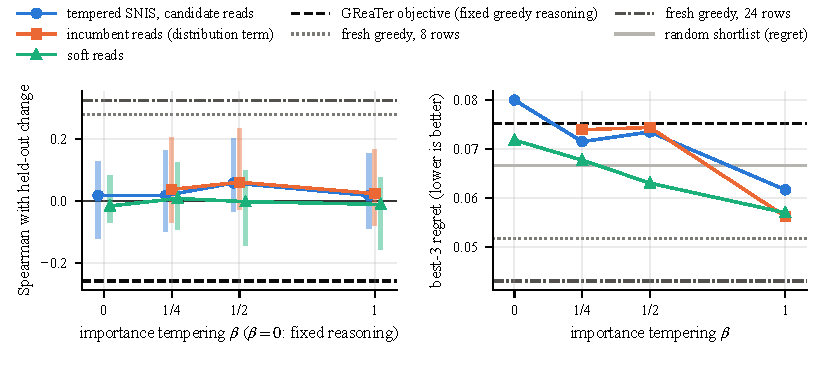
\includegraphics[width=0.85\linewidth]{figures/beta.pdf}
\caption{\textbf{Reweighting the incumbent's samples does not recover a ranking signal at any
tempering} (registered H-dist test, 11 pools; $\beta=0$: no reweighting). Left: pooled Spearman with
the held-out change for SNIS with candidate, incumbent (distribution term only) and soft reads;
bars: bias-corrected bootstrap ranges. Lines: the fixed-reasoning objective on the greedy reasoning
(\greater{} objective) and fresh greedy accuracy on $8$ and $24$ training questions (rows). Right:
best-3 regret (lower is better); random shortlist $0.067$.}
\label{fig:beta}
\end{figure}

\section{Verification budget decides}
\label{sec:exp-verify}
What an edit does must therefore be observed on fresh reasoning, a noisy instrument even under a
deterministic engine: if the fraction $f$ of questions whose correctness flips between two prompts
carries no systematic sign, their accuracy difference on $n$ questions has variance $f/n$, a
standard deviation of about $14$--$16$ points on $8$ questions and $3$ on $200$ at the flip rates of
single-token edits (Appendix~\ref{app:noise}). These analyses are exploratory; the matched-cost and
fixed-budget replays were specified after the registered outcome, the pipeline simulation of
Appendix~\ref{app:pipeline} before it. An edit is scored by its mean correctness change over the
incumbent on $G$ generations per candidate, greedy ($G$ questions) or sampled ($k$ samples at
$\tau=0.7$ on each of $r$ questions, $G=rk$; incumbent on the same seeds or on independent ones),
averaged over $400$ random subsets (Figure~\ref{fig:verify}).

\paragraph{Quality rises with generations, not with sampling or coupling.} Pooled Spearman rises
monotonically with $G$ for every verifier, from $+0.178$ for $4$ greedy reads to $+0.325$ for $24$
and $+0.413$ for $24\times4$ samples. At equal $G$, sampled reads rank worse than greedy ones in all
$15$ matched comparisons (by $0.03$--$0.06$, none significant alone), and common random numbers
\citep{corvelobenz2025coupled} change Spearman by at most $0.005$ over independent seeds, as
expected if edits rewrite the reasoning.

\paragraph{Small budgets lose accuracy.} Accepting the best edit whenever its verified change is
positive (verify-all) lowers held-out accuracy for every verifier with $G\le16$ ($-0.54$ to $-1.71$
points) and gains $0.41$ points with $24$ greedy reads (every sampled verifier at $G=24$ still loses
$0.21$--$0.58$) and $1.44$ at $G=96$. With fixed questions and another tie rule
(Appendix~\ref{app:pipeline}), $8$,
$16$ and $24$ greedy reads realize $-2.27$, $-0.77$ and $+1.14$ points: the losses at small budgets
are robust, the size of the gain at $G=24$ is not.

\paragraph{The acceptance rule limits the loss more than the allocation does.} A second replay fixes
the budget $B$ of candidate generations for one verification step (Appendix~\ref{app:verify},
Table~\ref{tab:margin}). Below the full budget, successive halving and a random shortlist of three
lose less than uniform verification ($0.68$--$1.57$ and $0.60$--$1.05$ points against
$1.09$--$1.90$), but neither gains at $B=480$ ($-0.24$, $-0.72$; uniform $+0.31$), and racing loses
at every budget; halving and racing follow budget-aware prompt selection
\citep{shi2024triple,schneider2025hbbops}. Under
uniform verification, accepting the best edit only if its paired gain exceeds two standard errors,
$2\sqrt{f/n}$ for the pool's flip rate $f$, keeps the loss at $0.24$--$0.62$ points for $B\le240$
and raises the full-budget gain to $+0.86$ points. Whether the
shortlist signal still matters under full verification is the question of \S\ref{sec:exp-search}.

\begin{figure}[t]
\centering
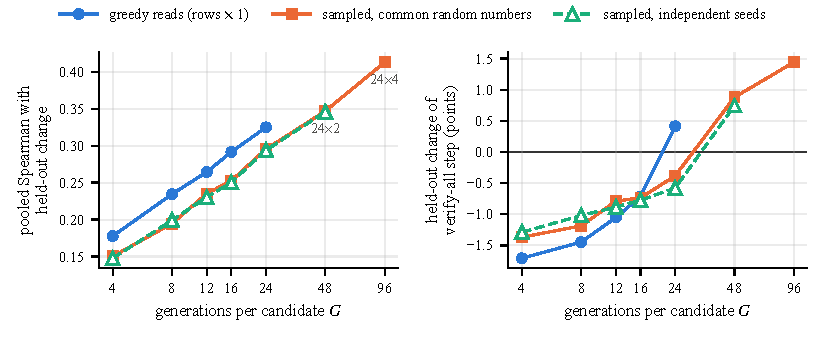
\includegraphics[width=0.85\linewidth]{figures/verify_cost.pdf}
\caption{\textbf{Verification quality is set by the number of fresh generations} (exploratory; 11
pools, 400 random question/sample subsets per cell). $G$: generations per candidate; rows: training
questions; sampled verifiers use one sample per question up to $24$ questions, then $24\times2$ and
$24\times4$. Left: pooled Spearman with the held-out change. Right: held-out change realized by a
verify-all step (ties broken uniformly).}
\label{fig:verify}
\end{figure}

\section{Self-optimization end to end}
\label{sec:experiments}

\subsection{End-to-end structural search}
\label{sec:exp-search}
End to end, task and optimizer model are \greater{}'s Llama-3-8B-Instruct and Gemma-2-9B-it, on its
21 BIG-Bench Hard tasks \citep{suzgun2023bbh} (50 train, 100 dev, up to 100 test questions), GSM8K
\citep{cobbe2021gsm8k} and FOLIO \citep{han2024folio}, split with a fixed seed; $41\%$ of our BBH
test questions were used to produce \greater{}'s published prompts, so comparisons with those prompts
are also reported on the clean remainder. The structural search (Algorithm~\ref{alg:search},
Appendix~\ref{app:search}) runs on Llama-3-8B and seven tasks (six BBH tasks and FOLIO) for $12$
rounds ($K=6$ proposals per slot, shortlist $3$), in arms that differ only in shortlist or
verification: patch-v50 (fixed-reasoning objective) and random-v50 (random shortlist), both verified
on all $50$ training questions, and random-v8 ($8$-question minibatches); textgrad-v50 (textual
gradients) is a different method class with its own proposals. The distributional
arm, registered conditional on H-dist or H-inc, is not run. The registered comparisons, paired by
seed within tasks, are patch-v50 vs.\ random-v50 (does the shortlist signal matter under full verification?) and
random-v50 vs.\ random-v8 (does the verification budget matter?); the prompt selected on dev is
evaluated on test once, with three numerical re-rolls (deterministic engine, $4{,}096$ tokens).
\todo{Seeds 1--3: test accuracy per task
and mean (full, clean); paired differences, conditional and task-level intervals, W/T/L;
textgrad-v50 (seeds 1--2); truncation; GPU time, tokens; the seven tasks.}

\subsection{Does \greater{} need its gradient?}
\label{sec:exp-greater}
The official \greater{} code (Llama-3-8B, our $50$ training questions, $106$ steps, top-$k$ $40$,
top-$q$ $6$, batch $64$; memory-only patches, Appendix~\ref{app:greater}) runs with its gradient
shortlist and with a shortlist drawn uniformly from the same model-proposed candidates, on tasks
fixed in advance because \greater{}'s published prompts gain most there: tracking shuffled objects
(five objects) and geometric shapes. \todo{Gradient vs.\ random shortlist: test accuracy of final
prompts (deterministic engine; full, clean) vs.\ the initial prompt; two registered repetitions per
arm (candidate sampling unseeded); wall time.}

\subsection{Breadth}
\label{sec:exp-breadth}
\todo{Configuration chosen end to end (random-v50 if it matches patch-v50) on 21 BBH tasks, GSM8K
and FOLIO, Llama-3-8B and Gemma-2-9B, vs.\ ZS-CoT and \greater{}'s initial and published prompts;
full and clean subsets; $4{,}096$ tokens; truncation and cost.}

\section{Related work}
\label{sec:related}

\paragraph{Gradient-based prompt optimization.} AutoPrompt \citep{shin2020autoprompt}, GCG
\citep{zou2023gcg} and PEZ \citep{wen2023hard} rank token substitutions by task-loss gradients
over relaxed prompt tokens; \greater{} \citep{das2025greater} takes this gradient after the model's
own reasoning, so a small model can optimize its own prompt without a stronger critic. One-hot
gradients poorly predict a token swap's loss change \citep{li2024fastergcg}, evaluation dominates
search cost \citep{zhao2024probe}, and policy-gradient methods score sampled prompts by reward on
fresh outputs \citep{deng2022rlprompt,diao2023bdpl}. Our exact objective still fails: the fixed
reasoning, not the linearization, limits it.

\paragraph{LLM-proposed and structural prompt optimization.} Most optimizers let a language model
propose candidates and decide by measured scores or critiques: APE \citep{zhou2023ape}, OPRO
\citep{yang2024opro}, ProTeGi \citep{pryzant2023protegi}, EvoPrompt \citep{guo2024evoprompt},
TextGrad \citep{yuksekgonul2025textgrad}, MIPRO in DSPy \citep{opsahl2024mipro,khattab2024dspy},
PromptWizard \citep{agarwal2025promptwizard} and GEPA \citep{agrawal2026gepa}. Textual gradients
improve prompts without behaving like gradients \citep{melcer2025textual}, random sampling is a
strong baseline \citep{lu2024strings}, and small models are weak optimizers in OPRO's loop
\citep{zhang2024revisiting}. Structure-aware variants edit sections or typed units (SAMMO, SPRIG,
SEPO, section-local textual gradients, segment-level optimization, prompt codebooks;
\citealp{schnabel2024sammo,zhang2024sprig,ma2026sepo,sharma2026mpo,kulin2026sapo,nath2026codebooks}),
and GMPO, GradPO and PMPO locate segments by gradients or masking
\citep{zhao2026gmpo,chakma2026gradpo,zhao2025pmpo}. Most judge edits on fresh outputs, often on
minibatches \citep{opsahl2024mipro,agrawal2026gepa}; we ask which selection signal a fixed proposer
needs, and how much verification.

\paragraph{Evaluation noise and prompt sensitivity.} Formatting changes move accuracy by tens of
points \citep{sclar2024formatspread,su2025single}; single-prompt evaluations rank models unreliably
\citep{mizrahi2024multiprompt}, prompt optimization changes rankings
\citep{sadjoli2025optimization} and its gains shrink with scale \citep{zhou2025scale}; greedy
decoding varies with batch size, kernels and serving stack
\citep{yuan2025nondeterminism,atil2025nondeterminism,he2025nondeterminism}. Budget-aware evaluation
casts prompt selection as best-arm identification or multi-fidelity search
\citep{shi2024triple,schneider2025hbbops}, estimates performance from few evaluations
\citep{polo2024prompteval} or selects informative subsets \citep{nian2026sess}; p1 separates
response noise from prompt-quality variance \citep{gao2026p1}, and \citet{gong2026why} ask which
edits help. Here a single-token edit moves accuracy on average like a numerical re-roll, and an
acceptance margin limits selection errors more than adaptive allocation does (exploratory).

\paragraph{Off-policy evaluation and importance sampling.} Importance sampling, the classical tool
of off-policy evaluation \citep{precup2000eligibility}, needs about $\exp(\mathrm{KL})$ samples
\citep{chatterjee2018sample}; Pareto smoothing diagnoses
heavy-tailed weights \citep{vehtari2024psis}, and the effective sample size is a loose proxy for
estimator quality \citep{elvira2022ess}; coupled randomness reduces the samples needed to compare
models \citep{corvelobenz2025coupled}. Our exact likelihood ratios fail a preregistered test, as
coverage predicts, and in exploratory replays common random numbers rank edits no better than
independent seeds. Appendix~\ref{app:related} covers off-policy methods for language models,
chain-of-thought faithfulness, attribution and block-wise contexts.

\section{Limitations}
\label{sec:limitations}
The validity pools use multiple-choice deduction and tracking tasks and one proposal procedure;
effects may differ for other answer types and proposal distributions, and the bootstrap intervals
are conditional on the pools (pool-level tests are the primary inference). Correctness of a
reasoning is judged by its extracted answer. The distributional score estimates accuracy under
temperature sampling, while benchmarks report greedy accuracy; the two agree in direction here but
need not in general. Importance weights over long reasoning are heavy-tailed; tempering trades
bias for variance and the effective-sample-size rule is a heuristic. The exact calculus and the
likelihood ratios require white-box access; the calculus assumes rotary position embeddings,
softmax attention and edits that tokenize cleanly at block boundaries. All experiments ran on
one or two shared 48\,GB GPUs with 8--9B models, which bounds seeds, tasks and model scale. Review
during the research process was done by a model of the same family as the one that ran it.


\subsection*{AI use statement}
% Authors: verify and adapt this statement before submission.
Generative AI was used extensively in this work. An autonomous coding agent (Claude, Anthropic),
directed by the authors, proposed and implemented the method, wrote the experiment and analysis
code, ran the experiments and drafted the text. Adversarial reviews of the idea and of intermediate
results were done by a model of a different family (GPT, OpenAI) in an early phase and later by
fresh-context instances of the same model family that read the code and raw results directly.
Related work was checked against the cited sources, and every numerical result is produced by
scripts that read the recorded run outputs. The authors reviewed all AI-assisted work and take
responsibility for the final content, including text, claims and artifacts.

\subsection*{Reproducibility statement}
Code for the superposed gated computation, the one-pass estimator, the distributional scores, the
search loop, all baselines and all analyses is provided as supplementary material and will be
released. Exactness propositions are proved in Appendix~\ref{app:proofs} and verified numerically
(Appendix~\ref{app:tests}); data splits are deterministic functions of the public \greater{}
release, and the released records list the example identifiers of every split, including the
questions used to form the clean subset; the preregistered experiment plan with its dated
amendments and all run records are included.

\bibliography{references}
\bibliographystyle{iclr2027_conference}

\appendix
\section{Exact calculus: illustration, proofs and the one-pass estimator}
\label{app:proofs}

\begin{figure}[h]
\centering
\resizebox{\textwidth}{!}{% Method overview: token-level relaxation (GReaTer) vs superposed typed blocks (GRAFT).
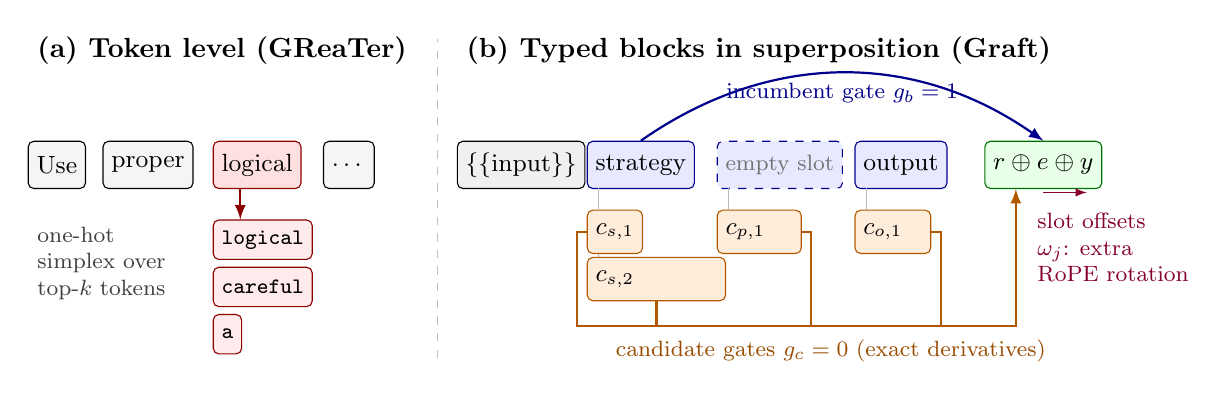
\begin{tikzpicture}[
  x=1cm, y=1cm, font=\small,
  box/.style={draw, rounded corners=2pt, minimum height=6mm, inner sep=3pt, anchor=west},
  tok/.style={box, fill=gray!8},
  alt/.style={box, fill=red!8, draw=red!55!black, minimum height=5mm, font=\footnotesize\ttfamily},
  frz/.style={box, fill=gray!12},
  inc/.style={box, fill=blue!9, draw=blue!55!black},
  cand/.style={box, fill=orange!14, draw=orange!70!black, minimum height=5.5mm},
  tail/.style={box, fill=green!9, draw=green!45!black},
  note/.style={font=\footnotesize, text=black!75, anchor=west, align=left},
  arr/.style={->, >=latex, thick},
]
% ---------------- (a) GReaTer ----------------
\node[anchor=west, font=\bfseries] at (0, 5.05) {(a) Token level (\greater{})};
\node[tok] (u) at (0, 3.6) {Use};
\node[tok] (pr) at (0.95, 3.6) {proper};
\node[tok, fill=red!12, draw=red!55!black] (lo) at (2.35, 3.6) {logical};
\node[tok] (re) at (3.75, 3.6) {\dots};
\node[alt] (a1) at (2.35, 2.65) {logical};
\node[alt] (a2) at (2.35, 2.05) {careful};
\node[alt] (a3) at (2.35, 1.45) {a};
\draw[arr, red!55!black] ([xshift=3.5mm]lo.south west) -- ([xshift=3.5mm]a1.north west);
\node[note] at (0, 2.35) {one-hot\\simplex over\\top-$k$ tokens};

\draw[gray!50, dashed] (5.2, 1.15) -- (5.2, 5.2);

% ---------------- (b) GRAFT ----------------
\node[anchor=west, font=\bfseries] at (5.45, 5.05) {(b) Typed blocks in superposition (\graft{})};
\node[frz] (x) at (5.45, 3.6) {\{\{input\}\}};
\node[inc] (s) at (7.1, 3.6) {strategy};
\node[inc, dashed, text=black!55] (p) at (8.75, 3.6) {\footnotesize empty slot};
\node[inc] (o) at (10.5, 3.6) {output};
\node[tail] (t) at (12.15, 3.6) {$r \oplus e \oplus y$};
% candidate lanes: each starts at its incumbent's first position
\node[cand] (c1) at (7.1, 2.75) {$c_{s,1}$};
\node[cand] (c2) at (7.1, 2.15) {$c_{s,2}$\,\rule{10mm}{0pt}};
\node[cand] (c3) at (8.75, 2.75) {$c_{p,1}$\,\rule{3mm}{0pt}};
\node[cand] (c4) at (10.5, 2.75) {$c_{o,1}$\,\rule{2mm}{0pt}};
\foreach \c in {c1, c3, c4} {\draw[gray!55] ([xshift=1.5mm]\c.north west) -- ++(0, 0.27);}
\draw[gray!55] ([xshift=1.5mm]c2.north west) -- ([xshift=1.5mm]c1.south west);
% incumbent gate
\draw[arr, blue!55!black] (s.north) to[out=35, in=145] node[pos=0.5, below, font=\footnotesize] {incumbent gate $g_b=1$} (t.north);
% candidate gates share a bus into the downstream tokens
\draw[orange!70!black, thick] (c1.west) -- ++(-0.12,0) |- (12.0, 1.55);
\foreach \c in {c3, c4} {\draw[orange!70!black, thick] (\c.east) -- ++(0.12,0) |- (12.0, 1.55);}
\draw[orange!70!black, thick] (c2.south) |- (12.0, 1.55);
\draw[arr, orange!70!black] (12.0, 1.55) -| ([xshift=4mm]t.south west);
\node[font=\footnotesize, text=orange!60!black, anchor=north] at (10.2, 1.5) {candidate gates $g_c=0$ (exact derivatives)};
\node[note, text=purple!70!black] at (12.7, 2.55) {slot offsets\\$\omega_j$: extra\\RoPE rotation};
\draw[->, >=latex, purple!70!black] (12.9, 3.25) -- (13.45, 3.25);
% The vertex and one-pass notes formerly drawn here are stated in the caption and in Section 3.
\end{tikzpicture}
}
\caption{\textbf{The instrument.} (a) \greater{} relaxes one prompt token over its top-$k$
substitutions; vertices keep the prompt's length and structure. (b) Candidate rewrites of each typed
block sit in parallel slots behind attention gates, with slot offsets as rotary rotations; every
vertex (replacement, deletion, insertion, combinations) is exactly an edited prompt
(Proposition~\ref{prop:vertices}), and one forward and backward pass scores every single-slot edit
(renormalized patching, Eq.~\ref{eq:patch}). Both hold the incumbent's reasoning $r$ fixed; edits
act mainly by changing $r$ (\S\ref{sec:theory}).}
\label{fig:overview}
\end{figure}

\paragraph{Setting.} We consider decoder-only transformers whose token mixing is
causal softmax attention with rotary position embeddings, possibly with logit
soft-capping and grouped-query attention; all other sublayers act on tokens
independently. We require that edits \emph{tokenize cleanly}: the edited prompt's
token sequence is the incumbent's prefix tokens, the candidate's tokens and the
incumbent's suffix tokens (edits violating this are excluded, which happens rarely
because blocks end at line breaks). Sliding windows are assumed to exceed the
sequence length, which our implementation asserts.

\paragraph{Proof of Proposition~\ref{prop:vertices}, base point.} By induction over layers we show that every
non-candidate token $t$ has the hidden state of the reference computation on
$P(x)\oplus r\oplus e\oplus y$. At the input, token identities and positions agree
($\Omega=0$). At a layer, the keys visible to $t$ are the non-candidate tokens that
precede it in the reference order, with gate $1$, and candidate tokens with gate
$0$. The latter contribute $0\cdot\exp(s_{tu}-m_t)=0$ to both the numerator and the
denominator of Eq.~\ref{eq:gate}; the max-shift $m_t$ may include them but softmax
is shift-invariant. Keys and values of the former equal the reference ones by the
induction hypothesis, and all other sublayers are tokenwise. \hfill$\square$

\paragraph{Proof of Proposition~\ref{prop:vertices}, edited prompts.} Fix a choice $e_j\in\{\text{keep},\text{delete},c_j\}$
per slot and let $P'$ be the edited prompt. Map every retained non-candidate token
$t$ and every chosen candidate token to its counterpart in $P'$. Its position in
$P'$ is its base position plus the cumulative length change of the edits before
it, $\sum_{k\prec t}(|e_k|-|b_k|)$, which is exactly $\pi_t+\Omega_t$ at
$\omega_k=|e_k|-|b_k|$ (candidates start at their slot's first position and move
only with earlier slots). The keys with non-zero gate visible to a mapped query are
exactly the tokens preceding it in $P'$: removed incumbents and unchosen
candidates have gate $0$; a chosen candidate of slot $j$ sees the prefix before
slot $j$ and the chosen candidates of earlier slots; a later token sees retained
incumbents and chosen candidates. Rotary scores depend only on position
differences, which agree with $P'$. The induction for the base point then applies
verbatim to the mapped tokens, so the loss equals $\ell(P';x,y,r)$. \hfill$\square$

\paragraph{Faithful reading.} The statement summarized in \S\ref{sec:theory}:

\begin{proposition}[Faithful reading]
\label{prop:faithful}
If, for every candidate $P'$, the answer read under $P'$ equals the answer read under $P$ except
on a set of reasonings of $\pi_P$-probability at most $\varepsilon$, then $|A|\le\varepsilon$ and
$J(P')-J(P)=D\pm\varepsilon$. Moreover, on a question whose reasoning $r$ supports a wrong answer
$a\neq y$, every decrease of the fixed-reasoning objective on $r$ raises the probability of reading
an answer that the reasoning does not support, and a decrease by $\delta>0$ nats implies
$q_{P'}(a\mid x,r)\le1-e^{\delta}q_P(y\mid x,r)$.
\end{proposition}

The proof is immediate from Eq.~\ref{eq:decomp} and $q_{P'}(a\mid x,r)+q_{P'}(y\mid x,r)\le1$.

\paragraph{Saturation of gate derivatives.} For one attention row, write the
current output as $o_0=N_0/Z_0$ with $N_0=\sum_{u\notin c}G_{tu}e^{s_{tu}-m}v_u$,
$Z_0=\sum_{u\notin c}G_{tu}e^{s_{tu}-m}$, and let $S_c=\sum_{u\in c}e^{s_{tu}-m}$,
$\bar v_c=S_c^{-1}\sum_{u\in c}e^{s_{tu}-m}v_u$. Then
$o(g)=\frac{N_0+gS_c\bar v_c}{Z_0+gS_c}$, so
\begin{equation*}
\frac{\partial o}{\partial g}\Big|_{0}=\frac{S_c}{Z_0}\,(\bar v_c-o_0),\qquad
o(1)-o(0)=\frac{S_c}{Z_0+S_c}\,(\bar v_c-o_0).
\end{equation*}
The first-order extrapolation exceeds the actual change by the factor
$1+S_c/Z_0$ in every head and layer, before any downstream nonlinearity. A
candidate block that competes with an instruction block already holding most of a
reading token's attention has $S_c/Z_0\gg1$, so raw gate derivatives are dominated
by attention mass rather than by the effect of the edit. The renormalized estimator
below uses $o(1)-o(0)$ exactly.

\paragraph{Renormalized patching.} Instead of gate derivatives, the one-pass estimator recomputes,
from the exact keys and values present in the superposed pass, each downstream attention output
with slot $j$ swapped to an alternative $a$ (query rotated by the length change), and linearizes
only the propagation through later layers:
\begin{equation}
\widehat{\Delta\ell}(a)=\sum_{\text{layers}}\sum_{t\text{ after slot }j}\big\langle\nabla_{o_t}\ell,\;o_t(a)-o_t(b_j)\big\rangle ,
\label{eq:patch}
\end{equation}
the AtP$^*$ principle \citep{kramar2024atp} applied to prompt edits. One forward and one backward
pass score every single-slot edit of a sequence. Its fidelity against exact scoring is reported in
\S\ref{sec:diagnosis} (mean Spearman $0.79$ between patched and exact objectives over the eleven
pools).

\section{Related work: faithfulness, attribution and block-wise contexts}
\label{app:related}
\paragraph{Off-policy methods for language models.} Off-policy prompt optimization has learned
reward models from logged data \citep{sun2024promptoirl} and smoothed weights over similar
sentences \citep{kiyohara2025logged}; Gumbel-max causal models generate counterfactual text
\citep{ravfogel2025gumbel,chatzi2025counterfactual}, and self-generated reasoning is a latent
variable in training \citep{zelikman2022star,phan2023trice}.

\paragraph{Faithfulness of chain-of-thought.} Explanations may not reflect how a model answers
\citep{turpin2023unfaithful}, answers depend on the reasoning to a varying degree
\citep{lanham2023faithfulness}, and a few forking, critical or decision tokens can decide the outcome
\citep{bigelow2025forking,lin2024critical,shen2026decision}. The fixed-reasoning objective rewards
unfaithful reads (Proposition~\ref{prop:faithful}), a channel too small to carry edit effects.

\paragraph{Attribution and block-wise contexts.} Attribution patching and AtP$^*$ \citep{syed2024atp,kramar2024atp}, ContextCite \citep{cohenwang2024contextcite},
AttriBoT \citep{liu2025attribot} and AT2 \citep{cohenwang2025at2} estimate the effect of parts of a
context; parallel context windows \citep{ratner2023pcw}, superposition prompting
\citep{merth2024superposition}, Prompt Cache \citep{gim2024promptcache}, Block-Attention
\citep{ma2025blockattention}, adaptive parallel encoding \citep{yang2025parallel} and EPIC
\citep{hu2025epic} encode or cache blocks independently with approximate positional handling. Our
superposed sequence differs in purpose and guarantee: candidate blocks compete for the same slot
behind gates, and continuous slot offsets make every vertex exactly the edited prompt, including
length-changing and combined edits, which is what lets the fixed-reasoning objective be computed
without approximation before it is tested.

\section{Numerical verification}
\label{app:tests}
All exactness claims are checked in fp32 on small randomly initialized models with a real
tokenizer and chat template. The base point and every replacement and deletion vertex are checked
on four architectures (Llama, Gemma-2 with attention and final logit soft-capping, OLMo-3 and
Qwen3); insertion into an empty slot and a combined vertex with three simultaneous edits of
different lengths on Llama, Gemma-2 and Qwen3. In all cases the superposed loss equals the loss of
the stock model on the real edited prompt to within $10^{-4}$ nats. Gate and offset gradients
agree with central finite differences to within $2\cdot10^{-3}+2\%$. The weighted rationale
objective, the decision margin and the tempered likelihood of a whole reasoning
($\tau=0.7$; base point and a vertex) match stock computations to $10^{-4}$, and renormalized
patching reconstructs the base computation to $10^{-4}$. A control confirms that approximate
right- and left-padded layouts are \emph{not} exact, so the tests detect the offset construction.
The exact teacher-forced likelihoods of whole reasonings used for the distributional scores are checked against a
direct per-token computation. The tests are part of the released code.

\section{Experimental details}
\label{app:details}

\paragraph{Prompts and proposals.} The initial prompt splits \greater{}'s instruction into
a strategy block (``Use proper logical reasoning and think step by step.''), an empty
procedure slot and an output block (``Finally give the actual correct answer.''). The
task model proposes candidates from two unlabeled training questions with a fixed
meta-prompt per operator (rewrite: rephrase, specialize, add a step, shorten, warn about a
pitfall, number the procedure, clarify the final answer; insert: procedure, verification,
organization of facts, common mistake, comparison of options, restating facts, strategy
hint, double-checking), sampled at temperature 0.8. Proposals are cleaned of preambles and
type labels and must tokenize cleanly at block boundaries.

\paragraph{Reader.} Greedy reasoning up to 1{,}024 tokens during search (384 in the validity
studies, with the truncation rates of \S\ref{sec:limitations}; 4{,}096 for dev selection and test),
stopped at the chat template's end-of-turn tokens; the extractor
is appended inside the assistant turn (``Therefore, the final answer is ('' for
multiple choice; ``(Yes or No) is:'' style for binary tasks; ``(a single integer) is:''
for counting and arithmetic); 16 greedy answer tokens (8 in the v3 validity runs, which predate the
reader fix) are parsed by answer type, tolerant
of Markdown emphasis and \LaTeX{} wrappers such as \verb|\boxed{}|. Qwen3 runs in
non-thinking mode. Rendered token ids are identical across the training-time and
evaluation engines for all three models.

\paragraph{Validity studies.} Per run: 2 training questions for proposals, 24 training
questions for predictors, 6 sampled reasonings per question (temperature 0.7) for forks, at most 3
forks per question, and 200 held-out questions for the target; seeds 101 (v3), 202 with a
non-initial state (v3), 303 (TS3). The validity tasks (logical deduction and tracking shuffled
objects with three and seven objects) are BBH tasks outside \greater{}'s 21; the benchmark of
\S\ref{sec:experiments} contains the five-object variants of both families. The exact objective takes one
pass per edited prompt. The paired bootstrap resamples training and
held-out questions jointly for all predictors (2{,}000 replicates) and keeps the proposal
pools fixed, so intervals are conditional on the pools; they are bias-corrected in
Table~\ref{tab:validity} and plain percentile intervals in Table~\ref{tab:validity-token}. The split-half
reliability $\kappa$ of each held-out target bounds the attainable correlation, roughly by
$\sqrt\kappa$ (Table~\ref{tab:validity}). The cost row of Table~\ref{tab:validity} counts seconds
per pool on one A6000, including the sampling that the fork predictors share.

\paragraph{Causal fork test.} For 32 training questions per run, forks are computed as in the
validity study. For each fork we force the correct-branch and the incorrect-branch token
after the shared prefix and sample six continuations each; the control forces, at a
uniformly random position of the shared prefix, the actual token versus the model's most
likely different token. Results are in Table~\ref{tab:causal}.

\section{Additional results}
\label{app:results}

\begin{table}[h]
\centering
\caption{\textbf{Token-level validity control:} single-token substitutions drawn from the
model's top-10 next tokens ($^t$), same training and held-out questions as the block runs
LD7/TS7 with seed 101. Columns as in Table~\ref{tab:validity}, except that the intervals are plain
percentile bootstrap intervals. The same edits are re-read under the deterministic engine in
Table~\ref{tab:reroll}.}
\label{tab:validity-token}
\resizebox{0.92\textwidth}{!}{\begin{tabular}{lrrrrrrr}
\toprule
Run & \makecell{Answer\\exact} & \makecell{Answer\\patch} & \makecell{Fork\\exact} & \makecell{Fork\\patch} & \makecell{Fresh\\8 rows} & \makecell{Fresh\\24 rows} & $\sqrt{\kappa}$ \\
\midrule
LD7-L$^t$ & -0.09 & +0.04 & +0.00 & +0.13 & +0.15 & +0.27 & 0.34 \\
LD7-Q$^t$ & +0.23 & +0.05 & -0.11 & -0.26 & -0.05 & -0.09 & 0.22 \\
TS7-L$^t$ & -0.27 & -0.29 & -0.08 & -0.13 & +0.15 & +0.17 & 0.31 \\
TS7-Q$^t$ & -0.25 & -0.45 & -0.16 & -0.13 & -0.07 & -0.10 & 0.51 \\
\midrule
Pooled & -0.10 & -0.16 & -0.09 & -0.10 & +0.04 & +0.06 & \\
95\% int. & \scriptsize[-0.22,+0.11] & \scriptsize[-0.27,+0.05] & \scriptsize[-0.28,+0.10] & \scriptsize[-0.26,+0.12] & \scriptsize[-0.15,+0.19] & \scriptsize[-0.14,+0.20] & \\
Cost (s) & 75 & 52 & 325 & 284 & 643 & 1254 & \\
\bottomrule
\end{tabular}
}
\end{table}

\subsection{Token edits and numerical re-rolls}
\label{app:reroll}

\begin{table}[h]
\centering
\caption{\textbf{Single-token edits versus numerical re-rolls of greedy decoding} (exploratory;
$200$ held-out questions, $384$-token budget, deterministic engine). Edits: the $24$ single-token
substitutions per pool of the token-level control (Table~\ref{tab:validity-token}). Re-rolls: the
unchanged prompt read in separate requests of $16$, $25$, $40$, $64$ and $100$ questions; the
accuracy columns and tests also count the base read (one request of all $200$ questions) as a
re-roll. Reasoning changed, correctness flipped: mean share of questions whose greedy reasoning or
correctness differs from the base read. sd: population standard deviation over reads. Permutation
$p$: exact two-sided test over all $\binom{30}{6}$ relabelings of edits and re-rolls, for the
difference of mean accuracies and the log ratio of accuracy variances; pooled: sum of per-pool
standardized statistics, $2\times10^5$ joint relabelings. TS7-Q reads hit the budget on
$99$--$100\%$ of questions.}
\label{tab:reroll}
\setlength{\tabcolsep}{4pt}% local to the enclosing table environment
\begin{tabular}{@{}lrrrrccrr@{}}
\toprule
 & \multicolumn{2}{c}{\makecell{Reasoning\\changed (\%)}} & \multicolumn{2}{c}{\makecell{Correctness\\flipped (\%)}} & \multicolumn{2}{c}{Accuracy (mean $\pm$ sd)} & \multicolumn{2}{c}{\makecell{Permutation\\$p$}} \\
\cmidrule(lr){2-3}\cmidrule(lr){4-5}\cmidrule(lr){6-7}\cmidrule(l){8-9}
Pool & Edits & Re-rolls & Edits & Re-rolls & Edits & Re-rolls & Mean & Variance \\
\midrule
LD7-L & 87.5 & 69.1 & 20.3 & 14.4 & $0.462 \pm 0.022$ & $0.467 \pm 0.018$ & 0.65 & 0.72 \\
TS7-L & 83.7 & 57.5 & 19.0 & 9.7 & $0.319 \pm 0.020$ & $0.301 \pm 0.022$ & 0.07 & 0.47 \\
LD7-Q & 92.9 & 84.6 & 14.6 & 15.8 & $0.521 \pm 0.020$ & $0.517 \pm 0.009$ & 0.69 & 0.09 \\
TS7-Q & 79.2 & 67.7 & 16.1 & 11.7 & $0.273 \pm 0.020$ & $0.271 \pm 0.009$ & 0.88 & 0.16 \\
\midrule
Pooled & & & & & & & 0.31 & 0.19 \\
\bottomrule
\end{tabular}

\end{table}

\begin{figure}[h]
\centering
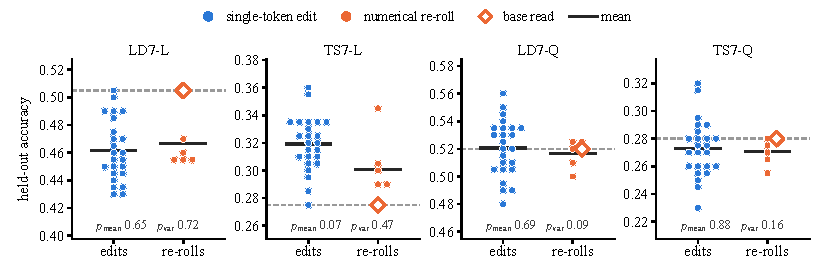
\includegraphics[width=\linewidth]{figures/reroll.pdf}
\caption{\textbf{Single-token edits and numerical re-rolls move held-out accuracy by similar
amounts} (exploratory). Each dot is one read on $200$ held-out questions: a single-token edit
(blue) or the unchanged prompt read in requests of a different size (orange). Diamond and dashed
line: the base read. Bars: means; the re-roll mean includes the base read. Every panel spans $13$
accuracy points. $p$: exact two-sided permutation tests for the mean and the variance
(Table~\ref{tab:reroll}).}
\label{fig:reroll}
\end{figure}

\paragraph{Details.} Figure~\ref{fig:reroll} shows every read of Table~\ref{tab:reroll}; the two
same-prompt re-reads per pool are token-identical to the base read. The tests compare the $24$
edits of a pool with six re-rolls (five chunked reads and the base read). The spread test has
little power with six re-rolls per pool: it does not detect a difference for Llama-3 ($p=0.72$,
$0.47$), and for Qwen3, where edits spread about twice as wide as re-rolls, it reaches $p=0.03$ only
for the two Qwen3 pools combined, a subset formed after seeing the data. Edits flip correctness on
more questions than re-rolls in three of the four pools (exact $p<3\times10^{-4}$), and the
additional flips cancel in accuracy.

\paragraph{A single greedy read is one draw.} On LD7-L the base read lies $3.5$ points above all
five chunked re-rolls ($0.505$ vs.\ $0.455$--$0.470$, sd $0.006$), so $23$ of $24$ edits score below
it. Leaving the base read out of the null (five re-rolls, all $\binom{29}{5}$ relabelings) gives mean
$p=0.86$, $0.22$, $0.67$, $0.75$ (pooled $0.22$) and variance $p=0.03$, $0.61$, $0.18$, $0.21$
(pooled $0.03$) for LD7-L, TS7-L, LD7-Q and TS7-Q: LD7-L edits then spread more than the five
tightly clustered re-rolls, and mean accuracies still agree. Edit accuracies spread close to or below what their
pairwise disagreement implies if each disagreement's sign were a fair coin (sample sd $0.022$,
$0.020$, $0.020$, $0.021$ against $0.024$, $0.024$, $0.020$, $0.021$); the Qwen3 re-rolls are
tighter than their disagreement implies ($0.010$ against $0.019$ and $0.010$ against $0.017$), so
the Qwen3 variance gap comes from the re-rolls rather than from unusually dispersed edits. First divergence
is the position of the first differing reasoning token; when one reasoning is a prefix of the
other, edits count the question at the shorter length and re-rolls leave it out, so the two
groups' medians are not directly comparable and we report them for edits only. Truncation was
recorded only for TS7-Q, where the base and re-roll reads hit the $384$-token budget on
$99$--$100\%$ of questions, so answers there are read off unfinished reasoning; it was not recorded
for the other three pools, whose incumbents' samples on the training questions are truncated at this
budget on $46\%$ (LD7-L), $14\%$ (TS7-L) and $100\%$ (LD7-Q).

\subsection{Read-off term per pool}

\begin{table}[h]
\centering
\caption{\textbf{The read-off term is small and unpredictive} (Eq.~\ref{eq:decomp}; eleven
pools; the incumbent's $16$ samples per training question, read under the incumbent and under
each candidate). Read-off flips: fraction of (candidate, question, sample) triples whose hard read
of the same reasoning changes; $|A|$: mean absolute read-off term per edit;
$|\Delta_{\text{held-out}}|$, $|\Delta_{\text{fresh}}|$: mean absolute change of held-out greedy
accuracy and of coupled fresh sampled accuracy on the training questions (accuracy points);
$\rho$: Spearman between $A$ and the held-out change; KL: median over edits of
$-\mathbb{E}_{\pi_P}\log w$ per reasoning (nats); sd$_x$: mean over edits of the within-question
standard deviation of $\log w$. Rows as in Table~\ref{tab:validity}; TS3-G: $A=0$ for every edit,
so $\rho$ is undefined.}
\label{tab:readoff}
\small
\begin{tabular}{lrrrr}
\toprule
Pool & Read-off flips & $|A|$ & $|D|$ & sd$(\log w)$ \\
\midrule
LD7, L$^\ast$ & 3.2\% & 0.012 & 0.034 & 43.5 \\
LD7, L & 1.4\% & 0.005 & 0.039 & 19.6 \\
LD3, L & 0.2\% & 0.002 & 0.041 & 19.0 \\
\bottomrule
\end{tabular}

\end{table}

Table~\ref{tab:readoff} gives the per-pool values summarized in \S\ref{sec:theory}: read-off flips
of $0.0$--$3.2\%$, $|A|$ of $0.0$--$1.2$ points against mean absolute held-out effects of
$2.1$--$10.9$, and
median divergences of $1.1$--$14.6$ nats per reasoning.

\subsection{Wrongly answered training questions}
\label{app:wrongrows}
Splitting training questions by whether the incumbent answers them correctly, and ranking each
question's loss changes across edits before averaging (which removes scale differences between
questions), the negative correlation of the fixed-reasoning objective on wrongly answered questions
persists for Llama-3 ($-0.25$ to $-0.61$ in all five pools) but not for Qwen3 ($+0.25$, $-0.04$,
$+0.07$; its other two pools have one wrongly answered question each); Gemma-2's pool gives
$-0.21$. This is consistent with the unfaithful-read mechanism of Proposition~\ref{prop:faithful}
for Llama-3; it does not show how much of the failure that mechanism accounts for.

\subsection{Failed repairs and an early pilot}

\begin{table}[h]
\centering
\caption{\textbf{Causal fork test.} Mean change in success probability when forcing the
correct instead of the incorrect fork token ($\Delta P_{\text{fork}}$), its absolute value,
and the absolute change at a random position of the shared prefix
($|\Delta P_{\text{ctrl}}|$).}
\label{tab:causal}
\small
\begin{tabular}{lrrrr}
\toprule
Run & Forks & $\Delta P_{\text{fork}}$ & $|\Delta P_{\text{fork}}|$ & $|\Delta P_{\text{ctrl}}|$ \\
\midrule
LD7-L & 41 & $+0.085$ & 0.199 & 0.191 \\
LD3-L & 41 & $+0.049$ & 0.203 & 0.246 \\
TS7-L & 47 & $+0.092$ & 0.220 & 0.234 \\
LD7-Q & 17 & $-0.069$ & 0.186 & 0.144 \\
LD3-Q & 11 & $+0.136$ & 0.258 & 0.146 \\
TS7-Q & 33 & $-0.025$ & 0.157 & 0.181 \\
\midrule
Pooled difference $|\Delta P_{\text{fork}}|-|\Delta P_{\text{ctrl}}|$ & \multicolumn{4}{r}{$-0.008$ [$-0.041,+0.026$]} \\
\bottomrule
\end{tabular}
\end{table}

\paragraph{Rationale-likelihood objective (pilot).} In an earlier pilot (validity v1; 8
training questions, 60 held-out questions; Llama-3 on date understanding and formal fallacies,
Gemma-2 on date understanding), the likelihood of a self-generated gold-consistent
rationale (PMPO-style) correlated $0.25$, $-0.16$ and $-0.02$ with the held-out change,
a correct-versus-incorrect rationale contrast $0.13$, $-0.22$, $-0.35$, and a policy-gradient
estimate $-0.30$ and $-0.49$; none was pursued. (The Gemma-2 pilot preceded a fix of its
end-of-turn token in sampling and is reported for completeness only.)

\paragraph{Answer-conditioned shortlist (H-cond).} Preregistered on the untouched task
TS3 before its data existed: scoring edits by the answer-loss change only on training questions
the incumbent answers correctly does not improve best-3 regret over the score on all questions ($+0.000$
[$-0.025,+0.021$]) and is worse than the exact expectation of a uniformly random ranking
($-0.029$ [$-0.048,-0.002$]). H-cond is retired.

\section{Reading, determinism and budgets}
\label{app:reader}
Greedy decoding is not reproducible across batch compositions and cached computation paths
\citep{yuan2025nondeterminism,he2025nondeterminism}. We found two sources in our generation
engine (vLLM). With prefix caching, same-prompt re-reads changed $2$--$14\%$ of answers, as large
as the end-to-end effects under study. Without prefix caching but with the engine core in a
separate process, the batch composition of the first decoding steps depends on when requests
arrive: a first check (three reads, $200$ questions) was token-identical, but with capped
concurrency one of two re-reads changed the greedy reasoning on $55$--$66\%$ of questions. With the
engine core in the calling process, so that all of a call's requests are enqueued before the first
step, four re-reads of $200$ questions were token-identical both at the evaluation configuration
($4{,}096$ tokens) and at the search memory configuration ($384$ tokens, a KV cache for about five
$4{,}096$-token sequences, so that sequences are preempted and recomputed). All end-to-end
evaluations, re-reads and re-roll measurements use this configuration, with one prompt's
questions per request in a fixed order. The validity studies' held-out targets
(\S\ref{sec:diagnosis}) were read by the Hugging Face model in the scoring process (batched greedy
generation with left padding; re-read reproducibility not measured), and the H-dist samples and
reads by the multiprocess vLLM engine without prefix caching (Gemma-2: Hugging Face)
\todo{re-read the held-out targets of the eleven pools with the in-process engine and report
the change of Table~\ref{tab:validity}}. Rendered token
ids are identical between the training-time (Hugging Face) and evaluation engines for all three
models. Reasoning budgets are $1{,}024$ tokens during search, $384$ in the validity studies and
$4{,}096$ for dev selection and test; truncation rates are reported (for the validity studies in
\S\ref{sec:limitations}).

\paragraph{Numerical re-rolls.} A reproducible engine is not batch-invariant. Reading the
unchanged incumbent in separate requests of $16$, $25$, $40$, $64$ or $100$ questions gives five
reads that are each reproducible but differ from the single-request base read and from each other.
In the four token pools the greedy reasoning differs from the base read on $67$--$71\%$ (LD7-L),
$56$--$61\%$ (TS7-L), $83$--$86\%$ (LD7-Q) and $65$--$73\%$ (TS7-Q) of questions, correctness on
$13$--$16\%$, $8$--$13\%$, $14$--$19\%$ and $10$--$13\%$, and accuracy over the six reads has
standard deviation $0.018$, $0.022$, $0.009$ and $0.009$. Batch-invariant kernels
\citep{he2025nondeterminism} would make these reads identical; we keep the engine and use its
re-rolls as the null against which edit effects are measured (\S\ref{sec:diagnosis},
Table~\ref{tab:reroll}).

\section{Distributional scores: protocol}
\label{app:dist}
Per pool (the records of \S\ref{sec:diagnosis}): $S=16$ reasonings for each of the $24$ training
questions under the incumbent, sampled at $\tau=0.7$ with no top-$k$/top-$p$ truncation (so that
the proposal is the full tempered softmax), the validity studies' $384$-token budget and a fixed
seed per (question, sample). For every candidate and sample, the tempered log-likelihood of the
reasoning is computed by teacher forcing in bfloat16 with float32 softmax, adding
$\log P(\text{stop})$ at the end of samples that stopped. Hard reads (greedy, $16$ tokens after the
extractor) and soft reads (gold-answer probability) are recorded under the incumbent and under
every candidate; four further samples per question under every prompt, with the same seed per
(question, sample), give the coupled fresh evaluation. No estimator generates reasoning under a
candidate. All estimators of Eq.~\ref{eq:snis} are computed afterwards from the stored values.
Tempering trades coverage for bias toward the fixed-reasoning family at $\beta=0$ (a smaller $\beta$
targets the geometric mixture $\pi_P^{1-\beta}\pi_{P'}^{\beta}$), and self-normalization hides the
failure of coverage: weights renormalized among samples that are all unlikely under the candidate
look well-conditioned.

\paragraph{Registered predictors.} Fixed before the data (Appendix~\ref{app:prereg}): the primary
predictor (Eq.~\ref{eq:snis} with candidate reads at a label-free $\beta^\ast$), the $\beta$ curve
$\{0,\tfrac14,\tfrac12,1\}$, soft reads, the first-order score-function estimate
$\widehat{\operatorname{Cov}}(\log w,c)$, effective-sample-size diagnostics, the coupled fresh
evaluation, the held-out targets and the kill criterion of \S\ref{sec:exp-validity}. The variant
with incumbent reads (H-inc, the distribution term alone) was defined after the first pool and is
confirmatory on pools $2$--$11$. $\beta^\ast$ is the largest $\beta\in\{1,\tfrac12,\tfrac14\}$
whose median per-question effective sample size $(\sum_s w_s^\beta)^2/\sum_s w_s^{2\beta}$ over
candidates is at least $S/4=4$ (else $\tfrac14$). It selected $\beta^\ast=\tfrac12$ in $8$ pools,
$\tfrac14$ in $2$ (TS7-L, TS3-G) and $1$ in $1$ (LD7-Q$^\ast$); at $\beta=1$ the median effective
sample size was $1.4$--$5.1$ of $16$. The label-free rule thus met its effective-sample-size
threshold in every pool, while in ten of the eleven pools the median divergence ($3.9$--$14.6$ nats
per reasoning) exceeded $\log 16$, the regime in which the coverage argument predicts failure with
$16$ samples. Verify-all for a predictor accepts the edit with the
largest positive predicted change and records its held-out change (zero if none is positive).

\begin{table}[h]
\centering
\caption{\textbf{Registered H-dist test (11 pools): estimates from the incumbent's own samples do
not predict the held-out change; fresh reasoning does.} Pooled Spearman: mean of the $11$ per-pool
Spearman correlations, with a $95\%$ percentile bootstrap interval over pools (pools resampled with
replacement, $20{,}000$ replicates), wider than the bias-corrected question-bootstrap intervals of
the text. Pools below random: best-3 regret strictly below the exact random expectation. Verify-all:
accept the edit with the highest positive predicted change (first listed among ties); mean realized
held-out change (points), pools improved/worsened (--: not simulated). \greater{} objective: the
fixed-reasoning objective (Eq.~\ref{eq:greater}) on the greedy reasoning. Rows: training questions;
sampled $24\times4$: four samples on each of the $24$ questions, with the incumbent read on the same
seeds. Candidate reads, $\beta=0$: the read-off term $A$ on the incumbent's samples. Primary: the
registered predictor ($\beta^\ast$ without labels). Incumbent reads: the distribution term alone,
all 11 pools (H-inc is confirmatory on pools 2--11). KL gate: primary if
$\mathrm{KL}\le\tfrac12\log16$, else fresh greedy on $8$ questions; $^\dagger$added after five
pools, before the Qwen3 and Gemma-2 data (a secondary analysis, Appendix~\ref{app:prereg}).
Figure~\ref{fig:beta} plots the
$\beta$ curves.}
\label{tab:hdist}
\small
\begin{tabular}{@{}lr@{\hspace{3pt}}lrcrc@{}}
\toprule
 & \multicolumn{2}{c}{\makecell{Pooled Spearman\\{}[pool bootstrap]}} & \makecell{Best-3\\regret} & \makecell{Pools below\\random} & \makecell{Verify-all\\(points)} & \makecell{Pools\\$+$/$-$} \\
\midrule
\multicolumn{7}{@{}l}{\textit{Fixed reasoning}} \\
\quad \greater{} objective (exact) & -0.258 & \scriptsize[-0.411, -0.095] & 0.075 & 4/11 & -5.00 & +1/-10 \\
\quad Candidate reads, $\beta=0$ & +0.018 & \scriptsize[-0.108, +0.156] & 0.080 & 4/11 & -- & -- \\
\midrule
\multicolumn{7}{@{}l}{\textit{Reweighted own samples}} \\
\quad SNIS, $\beta=1/4$ & +0.018 & \scriptsize[-0.193, +0.222] & 0.072 & 6/11 & -- & -- \\
\quad SNIS, $\beta=1/2$ & +0.058 & \scriptsize[-0.146, +0.252] & 0.073 & 6/11 & -- & -- \\
\quad SNIS, $\beta=1$ & +0.018 & \scriptsize[-0.177, +0.213] & 0.062 & 6/11 & -2.77 & +4/-7 \\
\quad Primary, $\beta^\ast$ & +0.034 & \scriptsize[-0.185, +0.241] & 0.075 & 6/11 & -2.18 & +5/-6 \\
\quad Incumbent reads, $\beta^\ast$ & +0.023 & \scriptsize[-0.212, +0.246] & 0.076 & 7/11 & -2.14 & +6/-5 \\
\quad First-order score function & -0.098 & \scriptsize[-0.285, +0.066] & 0.089 & 3/11 & -8.45 & +2/-9 \\
\quad KL gate$^\dagger$ & +0.218 & \scriptsize[+0.030, +0.382] & 0.052 & 8/11 & -- & -- \\
\midrule
\multicolumn{7}{@{}l}{\textit{Fresh reasoning}} \\
\quad Greedy, 8 rows & +0.277 & \scriptsize[+0.122, +0.404] & 0.052 & 9/11 & -2.27 & +3/-4 \\
\quad Greedy, 24 rows & +0.325 & \scriptsize[+0.173, +0.473] & 0.043 & 8/11 & +1.14 & +5/-4 \\
\quad Sampled, $24\times4$ (coupled) & +0.413 & \scriptsize[+0.242, +0.572] & 0.035 & 9/11 & +1.00 & +5/-5 \\
\midrule
Random shortlist & 0 &  & 0.067 & -- & -- & -- \\
\bottomrule
\end{tabular}

\end{table}

\paragraph{Further results.} As an acceptance rule, SNIS at $\beta=1$ loses $2.77$ held-out points
on average ($4$ pools improved, $7$ worsened; Table~\ref{tab:hdist}). The first-order score
function, the small-$\beta$ limit, is worse than random (best-3 regret $0.089$; gain $-0.023$
$[-0.041,-0.006]$). The primary score's agreement with the on-policy estimate of the same quantity
from fresh samples is $-0.52$ to $+0.36$ per pool. Coupled sampled accuracy on $24$ questions
$\times\,4$ samples has regret $0.035$ (gain over random $+0.031$ $[+0.026,+0.045]$, $9$ of $11$
pools).

\paragraph{Diagnostics added after five pools.} After the five Llama-3 pools and before any
Qwen3 or Gemma-2 data, descriptive diagnostics were added for all eleven pools: split-half
reliability of the primary score (samples $1$--$8$ against $9$--$16$), its agreement with the
coupled fresh estimate, the on-policy read-off term (Table~\ref{tab:readoff}), the divergence
$-\mathbb{E}_{\pi_P}\log w$ per reasoning, and a KL gate fixed from theory rather than data: an
edit is scored off-policy only if this divergence is at most $\tfrac12\log S=1.39$ nats, and
otherwise by fresh greedy accuracy on $8$ questions. The gate keeps $0$--$52\%$ of a pool's edits
off-policy (median $10\%$) and reaches a pooled Spearman of $+0.218$, below fresh-8 alone
($+0.277$). A numerical null re-scores the incumbent's samples with a different
batch size; the standard deviation of the log-ratio between the two passes measures bfloat16 and
padding noise. On the six pools sampled after the amendment it is $0.4$--$1.3$ nats per reasoning,
against within-question standard deviations of $\log w$ of $3.4$--$6.2$ nats on the same pools.

\paragraph{Intervals.} Bias-corrected bootstrap intervals resample training questions and
held-out questions within each pool and are conditional on the pools. For the coupled fresh
evaluation no replicate fell below the point estimate, so its interval ($[+0.415,+0.499]$)
excludes the estimate ($+0.413$).

\section{Pipeline simulation}
\label{app:pipeline}
For each pool and a verification size $n\in\{8,16,24\}$, one round of the shortlist-then-verify
loop is replayed from recorded per-question correctness: the edits are scored by a predictor on
the $24$ training questions, the top three (or all edits) are verified by fresh greedy accuracy on
the first $n$ training questions, and the best is accepted if it beats the incumbent on those
questions; the realized gain is the accepted edit's change on the $200$ held-out questions (zero if
none is accepted). Ties among candidates go to the first-listed edit, as in the verify-all column of
Table~\ref{tab:hdist}. The random shortlist is scored by its exact expectation over all
three-subsets. With a shortlist of three verified on $8$ questions, the answer-loss shortlist
realizes $-3.27$ (exact) and $-3.23$ (patched) points and a random shortlist $-1.34$; verifying all
edits on $8$, $16$ and $24$ questions realizes $-2.27$, $-0.77$ and $+1.14$; the best edit of each
pool would add $5.50$.

\section{Verification at matched cost: protocol}
\label{app:verify}

\paragraph{Noise of a paired comparison.}\label{app:noise} Fresh reasoning measures an edit's whole
effect, but greedy accuracy on $n$ questions is a noisy instrument even under a deterministic
engine: numerical re-rolls of the unchanged incumbent rewrite much of its greedy reasoning and move
its accuracy (\S\ref{sec:diagnosis}, Table~\ref{tab:reroll}). Counting flips gives the size of this
noise: comparing two prompts on $n$ questions, the accuracy difference is $(g-h)/n$ for $g$ gained
and $h$ lost questions, and if the $f=(g+h)/n$ flipped questions carry no systematic sign its
variance is $f/n$. From the measured disagreement between single-token edits this predicts a
standard deviation of $2.0$--$2.4$ points for their accuracies (observed: $2.0$--$2.2$).
Single-token edits flip $15$--$20\%$ of questions (Table~\ref{tab:reroll}), so comparing an edit
with the incumbent has a standard deviation of about $14$--$16$ points on $8$ questions, $5$--$6$ on
$50$ and $3$ on $200$, against mean block-edit effects of $2.1$--$10.9$ points. Selecting the best
of many candidates on such comparisons is a winner's curse: the largest verified gain is mostly
noise, and accepting it lowers held-out accuracy (\S\ref{sec:exp-verify}).

\paragraph{Protocol.} This analysis was added after the registered H-dist outcome and is exploratory. It uses the
eleven pools' recorded per-question correctness on the $24$ training questions: greedy reads of
every edit and of the incumbent, and four sampled reasonings per question and prompt at
$\tau=0.7$ that share one seed per (question, sample) across prompts (Appendix~\ref{app:dist}).
A verifier with $G$ generations per candidate predicts an edit's effect as the mean over questions
of candidate minus incumbent correctness, in one of three forms:
\emph{greedy} reads on $r$ questions ($G=r$, $r\in\{4,8,12,16,24\}$); \emph{coupled} sampled reads,
$k$ samples on each of $r$ questions with the incumbent read on the same $k$ seeds (common random
numbers; $G=rk$); and \emph{independent} sampled reads, as coupled but with the incumbent read on
$k$ other seeds of the four ($k\le2$), so that candidate and incumbent reads are independent. The
grid covers $rk\in\{4,8,12,16,24,48,96\}$ with $k\in\{1,2,4\}$ and $r\le24$; $G$ counts the
candidate's generations, since the incumbent's reads are shared by all candidates. For every cell
and pool, $400$ random draws of the $r$ questions (without replacement) and of the $k$ samples
give the expected Spearman correlation with the held-out change, the best-3 regret and the
realized held-out change of a verify-all step that accepts the edit with the largest predicted
change if it is positive (ties in the prediction broken uniformly in both).

\paragraph{Comparisons.} Pools are the units: coupled against greedy and coupled against
independent verification at equal $G$ are compared with exact sign-flip tests over pools. Greedy
verification has the higher mean Spearman at every equal $G$,
and no coupled-versus-greedy or coupled-versus-independent difference in Spearman reaches
$p<0.05$ (smallest $p=0.052$). Figure~\ref{fig:verify} plots the cells with one sample per question
and the $24\times2$ and $24\times4$ cells; mixed layouts fall in between (coupled $12\times2$:
$+0.281$). Because this analysis averages over question subsets while the pipeline simulation of
Appendix~\ref{app:pipeline} verifies on the first $n$ questions, verify-all on $8$ greedy
questions realizes $-1.45$ points here and $-2.27$ there (\S\ref{sec:exp-verify}).

\paragraph{Allocation and acceptance at a fixed budget.} A second replay, specified after the
results above and equally exploratory, uses the greedy reads of each pool's $K=20$ or $21$ edits
and of the incumbent on the $24$ training questions. The budget $B$ counts candidate reads of one
question; the incumbent's reads are shared and not counted. For every pool, budget and allocator,
$400$ random orders of the $24$ questions are drawn and the allocator reads questions in that
order. Unless a margin rule applies, it accepts its best candidate if the candidate's mean paired
correctness difference from the incumbent, on the questions it was read on, is positive (ties among
candidates broken uniformly). The score is the accepted edit's held-out change (zero if none),
averaged over orders and then over pools; accepting the best edit of every pool would gain $5.50$
points, and the mean edit changes held-out accuracy by $-2.93$. \emph{Uniform} verification reads
all $K$ edits on the first $\min(24,\lfloor B/K\rfloor)$ questions. The \emph{random shortlist}
reads three uniformly drawn edits on $\min(24,\lfloor B/3\rfloor)$ questions, the pattern of
Algorithm~\ref{alg:search} with a random shortlist. \emph{Successive halving} reads all edits on
$\max(1,\lfloor B/(K\lceil\log_2K\rceil)\rfloor)$ questions, keeps the better half by paired mean,
doubles the number of questions (reusing those already read) and repeats while the budget allows.
\emph{Racing} adds one question at a time to all surviving edits and, after $n$ questions, drops
every edit whose paired mean lies more than $\sqrt{2f/n}$ below the leader's, until one edit
remains, the budget is spent or all questions are read. Here $f$ is the pool's flip rate, the
fraction of (edit, question) pairs whose correctness differs from the incumbent's ($0.06$--$0.41$
across pools); it is computed once per pool from all recorded reads, where a verifier would
estimate it from earlier rounds. The
\emph{margin} rules verify uniformly but accept only if the paired gain exceeds $c\sqrt{f/n}$ with
$c=1$ or $2$, the standard error of a mean of $n$ paired differences of which a fraction $f$ is
non-zero (see the noise paragraph above); at $24$ questions the $2$-SE margin is $10$--$26$ accuracy points.

\begin{table}[h]
\centering
\caption{\textbf{Held-out change (points) realized by one verification step at a fixed budget}
(exploratory; 11 pools, 400 question orders each). $B$: candidate reads of one question, the
incumbent's reads not counted. Rows per edit: training questions read per edit, $\lfloor
B/K\rfloor$ for $K=20$--$21$ edits, at most $24$. Margin rules: uniform verification, accepting only if the paired gain exceeds $1$ or $2$
standard errors $\sqrt{f/n}$. Best edit of each pool: $+5.50$; mean edit: $-2.93$.}
\label{tab:margin}
\small
% Generated from D:/Company/research-artifacts/graft-runs/dist-final/racing_sim.json
% (scripts/research/graft/racing_sim.py): 100 * cells[B][allocator].mean; rows per edit = floor(B/K), K = 20-21.
\begin{tabular}{@{}lrrrrrrr@{}}
\toprule
Budget $B$ & 40 & 60 & 80 & 120 & 160 & 240 & 480 \\
Rows per edit (uniform) & 1--2 & 2--3 & 3--4 & 5--6 & 7--8 & 11--12 & 22--24 \\
\midrule
Uniform & -1.70 & -1.90 & -1.60 & -1.66 & -1.39 & -1.09 & +0.31 \\
Random shortlist of 3 & -1.05 & -0.75 & -0.75 & -0.60 & -0.79 & -0.78 & -0.72 \\
Successive halving & -1.57 & -1.07 & -0.99 & -1.01 & -1.03 & -0.68 & -0.24 \\
Racing & -1.83 & -1.94 & -1.68 & -1.52 & -1.50 & -1.24 & -1.09 \\
\midrule
Uniform, gain $>1$ SE & -1.73 & -1.49 & -0.87 & -1.04 & -1.13 & -0.96 & -0.07 \\
Uniform, gain $>2$ SE & -0.45 & -0.62 & -0.35 & -0.38 & -0.24 & -0.43 & +0.86 \\
\bottomrule
\end{tabular}

\end{table}

\paragraph{Results.} Below the full budget every allocator loses held-out accuracy
(Table~\ref{tab:margin}). Successive halving and the random shortlist, which compare fewer
candidates on more questions each, lose less than uniform verification there, but at $B=480$ only
uniform verification gains among the four allocators without a margin ($+0.31$; halving $-0.24$,
shortlist $-0.72$, racing $-1.09$). This
uniform value differs from verify-all on $24$ greedy reads ($+0.41$, Figure~\ref{fig:verify})
because the two pools with $21$ edits read $22$ questions and ties are drawn anew. The $2$-SE margin
has the smallest loss at every budget below $480$, losing less than uniform verification in $6$ or
$7$ of the $11$ pools at each of these budgets, and the largest gain at $B=480$. There every edit is
read on all or nearly all questions, so each pool contributes essentially one decision: the margin
leaves seven pools unchanged, in which uniform verification gained in two and lost in three, and
one pool contributes $+10.5$ points under both rules. A $1$-SE margin is too small: it loses
$0.87$--$1.73$ points below the full budget and $0.07$ at it.

\section{Distributional self-optimization of structured prompts}
\label{sec:method}

\begin{algorithm}[t]
\caption{Structural shortlist-then-verify search (one round); arms differ only in line 4}
\label{alg:search}
\begin{algorithmic}[1]
\Require model $f_\theta$, typed incumbent $P$, training questions $D$ ($|D|=50$), scoring
questions $D_s\subset D$, shortlist size $\mu$
\State propose $K$ label-free candidates per slot with $f_\theta$ from unlabeled questions
\State keep edits that tokenize cleanly at block boundaries and preserve required literals
\State \textbf{if} no samples for $P$: draw $S$ reasonings per $x\in D_s$ under $P$ at temperature $\tau$; read them under $P$
\State score every edit: \textsc{dist}: $\widehat\Delta_{\beta^\ast}$ (Eq.~\ref{eq:snis}) from exact $\log w$ on the shared samples;
\Statex \hspace{1.2em} controls: \greater{}'s objective (one pass, \S\ref{sec:calculus}); exact fixed-reasoning loss; random
\State regenerate greedy reasoning on all of $D$ for the top-$\mu$ edits
\State accept the best if it makes fewer errors on $D$ than $P$ (ties: answer loss)
\end{algorithmic}
\end{algorithm}

Algorithm~\ref{alg:search} lifts \greater{}'s loop to blocks. As in \greater{}, the model proposes
candidates, a signal shortlists them, and fresh reasoning on all training questions decides; the
model optimizes its own prompt and supervision enters only through correctness. \textsc{dist}
replaces the shortlist signal by the distributional score: $S$ reasonings per scoring question are
sampled once per incumbent and reused while it stays the incumbent, so the per-round cost is one
teacher-forced pass per candidate and sample; nothing is generated under candidates before
verification. $\beta^\ast$ is chosen per round from the effective sample size (\S\ref{sec:theory}).
The controls isolate the shortlist signal: \greater{}'s objective lifted to blocks (patched, the
one-pass estimate; exact, one pass per edit), a uniformly random shortlist drawn from its own
random stream (minibatches and proposals are identical across arms for a seed), and a
textual-gradient arm in which the same model critiques failed training questions and rewrites
each block (a different method class, not a matched-pool control). Dev questions select among the
incumbents at four evenly spaced rounds; the selected prompt is read once on test.

\paragraph{Reading.} Every prompt in a comparison is read by one engine with identical
token-level rendering: greedy reasoning, the task-typed extractor inside the assistant turn and
$16$ greedy answer tokens parsed by answer type. The engine is configured to be deterministic
(no prefix caching; one prompt's questions per request), which we verified by repeated reads;
reasoning budgets are $1{,}024$ tokens during search and $4{,}096$ for dev selection and test, and
truncation rates are reported.


\section{Official \greater{} on one GPU}
\label{app:greater}
We run the official \greater{} code with Llama-3-8B on our $50$ training questions of each task,
copied verbatim from \greater{}'s own data files in our seeded order, with $106$ steps, top-$k$
$40$, top-$q$ $6$ and batch $64$. The released configuration loads the model twice, for a
gradient worker and for a reasoning worker; we have one $48$\,GB GPU.
Our patches change only where tensors live and when they are freed: (i) one local copy of the
model serves both workers; (ii) the reasoning worker regenerates the training questions in calls
of one eighth of them instead of one half, and every question is still evaluated; (iii) candidate
logits (computed in \greater{}'s default batches of $9$) are freed before the next candidate is
evaluated; (iv) the gradient
worker's weights are frozen and its CUDA cache is emptied after each task. Freezing removes about
$16$\,GB of weight gradients that \greater{}'s backward pass computed but never read; the gradient
with respect to the one-hot prompt tokens, the only one used, is unchanged. The optimization
algorithm, its hyperparameters, the evaluation of candidates by fresh reasoning and the selection
rule are unchanged; smaller generation calls change batch shapes, which perturbs greedy decoding
numerically as any change of batch size does (Appendix~\ref{app:reader}). A two-step smoke run
took $31$ minutes with a peak of $33$\,GB. The patches are released with our code.

\paragraph{Shortlist ablation.} One environment switch replaces the gradient ranking and nothing
else: instead of the $q$ candidates with the largest gradient score among the model's $k$ proposed
tokens, the shortlist is $q$ of the same $k$ proposals drawn uniformly at random, and the gradient
is not computed. Regeneration, scoring by fresh reasoning and selection are identical in both
arms. The ablation was registered before its runs (Appendix~\ref{app:prereg}).
\todo{runs: tracking shuffled objects (five objects) and geometric shapes, gradient and random
shortlist; test accuracy under the deterministic engine, full and clean subsets; wall time.}

\section{Preregistration and amendments}
\label{app:prereg}
The experiment plan was fixed before any optimizer result and amended with dates and
reasons (Stage C is the end-to-end structural search of \S\ref{sec:exp-search}): dev selection
restricted to checkpoint incumbents; Stage C deferred until the
validity study; H-fork and its replication protocol frozen after one exploratory result;
evaluation separated from search with one shared engine; a reader fix (\LaTeX{}-wrapped
answers, answer length and reasoning budget) before any baseline or Stage C result; the
Stage C variant set and its later re-scoping to 140 runs before any Stage C outcome;
H-cond before its data; and the official \greater{} shortlist ablation before its runs.
After an internal review found the generation engine nondeterministic (prefix caching) and a
truncation artifact, the reading protocol was fixed for every later evaluation read (no prefix caching, one
prompt's questions per request, a $4{,}096$-token budget for re-reads, dev selection and test),
proposals cut at their token cap were discarded, pool-level tests became primary, and the
distributional hypothesis H-dist with its kill criterion was fixed before any of its data; its
incumbent-read variant H-inc was defined after the first of eleven pools and is tested on the other
ten. The Stage C protocol was then revised to verify on all $50$ training questions (as \greater{}
does) before any of its runs. After five of the eleven H-dist pools, before any Qwen3 or Gemma-2
data, descriptive diagnostics, a KL gate fixed from theory and a numerical null were added
(Appendix~\ref{app:dist}), and the coverage prediction of \S\ref{sec:theory} was first written down.
When a second source of nondeterminism appeared (request timing with a
multiprocess engine core), all evaluation, re-read and re-roll jobs and the Stage C search moved to
the in-process engine, and the one Stage C run made before the change was archived and re-run.
After the registered H-dist and H-inc outcomes, four analyses were added and are labelled
exploratory: verification at matched generation budgets, allocation and acceptance at a fixed
budget (both Appendix~\ref{app:verify}; the latter is not logged in the plan), numerical re-rolls as
the null for edit effects (\S\ref{sec:diagnosis}), and truncation of held-out reads and of the
H-dist samples. The pool-level sign-flip tests of the validity study (\S\ref{sec:diagnosis}) were
made primary after all eleven validity pools existed. The failed hypotheses (H-fork, H-cond, H-dist, H-inc) are reported as
registered.
Deviations: the v3 replication runs on a non-initial prompt state share their $200$ held-out
questions with the initial-state run of the same task and model (the protocol asked for
independent slices), and the bootstrap does not resample pools; under the stricter preregistered
causal statistic (signed $\Delta P_{\text{fork}}-|\Delta P_{\text{ctrl}}|=-0.156$
[$-0.203,-0.112$]) H-fork fails as under the lenient one. Table~\ref{tab:validity} reports best-3
regret, registered for TS3, instead of the best-5 regret registered for the v3 pools; under best-5
the patched objective's regret ($0.069$) also exceeds that of the random ranking then used
($0.056$). The token-level re-roll study (Table~\ref{tab:reroll}) re-reads at the validity budget of
$384$ tokens rather than the registered $4{,}096$, to match Table~\ref{tab:validity-token}.




\end{document}
